%%%%%%%%%%%%%%%%%%%%%%%%%%%%%%%%%%%%%%%%%%%%%%%%%%%%%%%%%%%%
%%  This Beamer template was created by Cameron Bracken.
%%  Anyone can freely use or modify it for any purpose
%%  without attribution.
%%
%%  Last Modified: January 9, 2009
%%

\documentclass[xcolor=x11names,compress,ignorenonframetext]{beamer}

%% General document %%%%%%%%%%%%%%%%%%%%%%%%%%%%%%%%%%
\usepackage{graphicx}
\usepackage{tikz}
\usepackage[abs]{overpic}
\usepackage{pict2e}

%\usetikzlibrary{decorations.fractals}

\renewcommand{\star}{*}

\DeclareMathOperator*{\argmin}{arg\,min}
\DeclareMathOperator{\gap}{gap}

\def\rf{\mathrm{F}}
\def\bigbar{\big\|}
\def\pinv{\dagger}
\def\transp{^T}
% 
\newcommand{\samats}[1]{\ensuremath{\mathbb{M}^{#1}_{\mathrm{sa}}}}
\newcommand{\s}{\sigma} % singular values
\newcommand{\asymO}[1]{\ensuremath{\mathop{\text{O}}\!\left(#1\right)}}
\DeclareMathOperator{\sgn}{sgn}

\newcommand{\norm}[1]{\ensuremath{\left\|#1\right\|}}
\newcommand{\supoverinfball}{\ensuremath{\max_{\infnorm{\mat{u}} = 1}}}
\newcommand{\supovertball}{\ensuremath{\max_{\norm{\mat{u}}_2 = 1}}}
\newcommand{\supoverqball}{\ensuremath{\max_{\qnorm{\mat{u}} = 1}}}
\newcommand{\eqqcolon}{=\mathrel{\mathop:}} %this may not be what I want, =:

\newcommand{\mat}[1]{\ensuremath{\mathbf{#1}}}
\renewcommand{\vec}[1]{\ensuremath{\mathbf{#1}}}
\newcommand{\e}{\ensuremath{\mathrm{e}}}
\newcommand{\E}{\ensuremath{\mathbb{E}}}
\newcommand{\Prob}[1]{\ensuremath{\mathbb{P}\left\{#1\right\}}}
\newcommand{\CondProb}[2]{\ensuremath{\mathbb{P}\left\{#1 \,\left|\, #2 \right.\right\}}}
\newcommand{\lnorm}[2]{\ensuremath{\left\| #2 \right\|_{L_{#1}}}}
\newcommand{\lipnorm}[1]{\ensuremath{\left\| #1 \right\|_\Pi}}
\newcommand{\R}{\ensuremath{\mathbb{R}}}
\newcommand{\Cfield}{\ensuremath{\mathbb{C}}}
\newcommand{\randcon}{\ensuremath{\Psi}}
\newcommand{\indicator}[1]{\ensuremath{\mathbb{1}\left\{#1\right\}}}

\newcommand{\xiNorm}[1]{\ensuremath{\left\|#1\right\|_\xi}}
\newcommand{\TNorm}[1]{\ensuremath{\left\|#1\right\|_2}}
\newcommand{\TNormS}[1]{\ensuremath{\left\|#1\right\|_2^2}}
\newcommand{\FNorm}[1]{\ensuremath{\left\|#1\right\|_\mathrm{F}}}
\newcommand{\FNormS}[1]{\ensuremath{\left\|#1\right\|_\mathrm{F}^2}}
\newcommand{\VTNorm}[1]{\ensuremath{\left\|#1\right\|_2}}
\newcommand{\VTNormS}[1]{\ensuremath{\left\|#1\right\|_2^2}}
\newcommand{\tracenorm}[1]{\ensuremath{\trace\left(#1\right)}}

\newcommand{\xinorm}[1]{\ensuremath{\big\|#1\big\|_\xi}}
\newcommand{\xinorms}[1]{\ensuremath{\big\|#1\big\|_\xi^2}}
\newcommand{\snorm}[1]{\ensuremath{\left\|#1\right\|_2}}
\newcommand{\snorms}[1]{\ensuremath{\big\|#1\big\|_2^2}}
\newcommand{\fnorm}[1]{\ensuremath{\left\|#1\right\|_{\mathrm{F}}}}
\newcommand{\fnorms}[1]{\ensuremath{\big\|#1\big\|_{\mathrm{F}}^2}}
\newcommand{\mcnorm}[1]{\ensuremath{\big\|#1\big\|_{\mathrm{mc}}}}
\newcommand{\mcnorms}[1]{\ensuremath{\big\|#1\big\|_{\mathrm{mc}}^2}}

\newcommand{\pnorm}[1]{\ensuremath{\left\|#1\right\|_p}}
\newcommand{\qnorm}[1]{\ensuremath{\left\|#1\right\|_q}}
\newcommand{\infnorm}[1]{\ensuremath{\left\|#1\right\|_\infty}}
\newcommand{\infonorm}[1]{\ensuremath{\left\|#1\right\|_{\infty\rightarrow 1}}}
\newcommand{\inftnorm}[1]{\ensuremath{\left\|#1\right\|_{\infty\rightarrow 2}}}
\newcommand{\onetwonorm}[1]{\ensuremath{\left\|#1\right\|_{1 \rightarrow 2}}}
\newcommand{\twoinfnorm}[1]{\ensuremath{\left\|#1\right\|_{2 \rightarrow \infty}}}
\newcommand{\smalltwoinfnorm}[1]{\ensuremath{\|#1\|_{2 \rightarrow \infty}}}
\newcommand{\infone}{\ensuremath{\infty\!\rightarrow\!\!1}}
\newcommand{\inftwo}{\ensuremath{\infty\!\rightarrow\!\!2}}
\newcommand{\infp}{\ensuremath{\infty\!\rightarrow\!p}}
\newcommand{\twoinf}{\ensuremath{2\!\!\rightarrow\!\!\infty}}
\newcommand{\colnorm}[1]{\ensuremath{\left\|#1\right\|_{\mathrm{col}}}}
\newcommand{\rownorm}[1]{\ensuremath{\left\|#1\right\|_{\text{\rmfamily{row}}}}}
\newcommand{\cutnorm}[1]{\ensuremath{\left\|#1\right\|_{\text{\rmfamily{C}}}}}

\newcommand{\F}{F}
\newcommand{\lambdamax}[1]{\ensuremath{\lambda_{\mathrm{max}}\left(#1\right)}}
\newcommand{\lambdamin}[1]{\ensuremath{\lambda_{\mathrm{min}}\left(#1\right)}}
\newcommand{\sigmamin}[1]{\ensuremath{\sigma_{\mathrm{min}}\left(#1\right)}}
\newcommand{\sigmamax}[1]{\ensuremath{\sigma_{\mathrm{max}}\left(#1\right)}}
\newcommand{\Isom}[2]{\ensuremath{\mathbb{V}_{#1}^{#2}}}
\DeclareMathOperator{\tr}{tr}
\DeclareMathOperator{\trace}{Tr}
\DeclareMathOperator{\rank}{rank}
\DeclareMathOperator{\var}{Var}
\newcommand{\trbrace}[1]{\ensuremath{\tr\left(#1\right)}}
\newcommand{\trexp}[1]{\ensuremath{\tr\exp\left(#1\right)}}
\newcommand{\const}[1]{\ensuremath{\mathrm{#1}}}

%\newtheorem{thm}{Theorem}[chapter]
%\newtheorem{prop}[thm]{Proposition}
%\newtheorem{lemma}[thm]{Lemma}
%\newtheorem{cor}[thm]{Corollary}
%\newtheorem{defn}[thm]{Definition}

%\theoremstyle{remark}
%\newtheorem{remark}[thm]{Remark}


% Bunch of stuff from the SRHT paper, need to eliminate redundancy and fold in
\newcommand{\Probab}[1]{\mbox{}{\mathbb{P}}\left(#1\right)}
\newcommand{\Exp}{\mbox{}{\mathbf{E}}}
\newcommand{\Expect}[1]{\mbox{}{\mathbb{E}}\left[#1\right]}
\newcommand{\Varnce}[1]{\mbox{}{\mathbf{Var}}\left[#1\right]}
\newcommand{\Trace }[1]{\mbox{}{\mathrm{Tr}}\left(#1\right)}
\newcommand{\diag  }[1]{\mbox{}{\textrm{diag}}\left(#1\right)}
\newcommand{\Sqrt  }[1]{\mbox{}\left(#1\right)^{1/2}}
\newcommand{\Qdrt  }[1]{\mbox{}\left(#1\right)^{1/4}}
\newcommand{\FNormB }[1]{\mbox{}\left\|#1\right\|_{\mathrm{F}}  }
\newcommand{\FNormBS}[1]{\mbox{}\left\|#1\right\|_{\mathrm{F}}^2}
\newcommand{\FNormF}[1]{\mbox{}\|#1\|_\mathrm{F}^4}
\newcommand{\FNormQ}[1]{\mbox{}\left\|#1\right\|_\mathrm{F}^4}
\newcommand{\TNormB }[1]{\mbox{}\left\|#1\right\|_2  }
\newcommand{\TNormBS}[1]{\mbox{}\left\|#1\right\|_2^2}
\newcommand{\TNormF}[1]{\mbox{}\|#1\|_2^4}
\newcommand{\TNormQ}[1]{\mbox{}\left\|#1\right\|_2^4}
\newcommand{\XNormB }[1]{\mbox{}\left\|#1\right\|_{\xi}  }
\newcommand{\XNormBS}[1]{\mbox{}\left\|#1\right\|_{\xi}^2}
\newcommand{\XNorm }[1]{\mbox{}\|#1\|_{\xi}  }
\newcommand{\XNormS}[1]{\mbox{}\|#1\|_{\xi}^2}
\newcommand{\PNorm }[1]{\mbox{}\|#1\|_{p}  }
\newcommand{\PNormS}[1]{\mbox{}\|#1\|_{p}^2}
\newcommand{\XNormQ}[1]{\mbox{}\left\|#1\right\|_{\xi}^4}
\newcommand{\VTNormQ}[1]{\mbox{}\left|#1\right|^4}
\newcommand{\VTTNorm }[1]{\mbox{}\left|#1\right|_2  }
\newcommand{\VTTNormS}[1]{\mbox{}\left|#1\right|_2^2}
\newcommand{\VTTNormQ}[1]{\mbox{}\left|#1\right|_2^4}
\newcommand{\MCNorm}[1]{\mbox{}\|#1\|_{1 \rightarrow 2}}
\newcommand{\MCNormS}[1]{\mbox{}\|#1\|_{1 \rightarrow 2}^2}
\newcommand{\INorm}[1]{\mbox{}\|#1\|_\infty}

\newcommand{\qedsymb}{\hfill{\rule{2mm}{2mm}}}

\newcommand{\dvc}{\ensuremath{d_{\small \sf VC}}}
\newcommand{\abs }[1]{\left|#1\right|}
\newcommand{\EE}[1]{\ensuremath{\mathbb{E}\left[#1\right] } }
\newcommand{\condE}[2]{\ensuremath{\mathbb{E}\left[#2 \,\left|\, #1 \right.\right]}}

\def\gammab{{\bm{\gamma}}}
\def\kappab{{\bm{\kappa}}}
\def\sig{{\bm{\Sigma}}}
\def\sigplus{{\bm{\Sigma}^{+}}}
\def\siginv{{\bm{\Sigma}^{-1}}}
\def\bet{{\bm{\beta}}}
\def\one{{\bm{1}}}
\def\exp{\ensuremath{\mathrm{exp}}}
\def\rank{\mathrm{rank}}
\newcommand{\stablerank}[1]{\operatorname{sr}\left(#1\right)}

%\def\cond{\hbox{\rm \mathbf{k}}}

\def\col{\hbox{\mathrm{col}}}
\def\ker{\hbox{\mathrm{ker}}}
\def\ahat{{\hat\a}}
\def\b{{\mathbf b}}
%\def\e{{\mathbf e}}
\def\expe{\mathrm{e}}
\def\q{{\mathbf q}}
\def\rb{{\mathbf r}}
%\def\s{{\mathbf s}}
%\def\u{{\mathbf u}}
\def\v{{\mathbf v}}
\def\x{{\mathbf x}}
\def\y{{\mathbf y}}
\def\z{{\mathbf z}}
\def\h{{\mathbf h}}
\def\d{{\mathbf \delta}}
\def\xhat{{\hat\x}}
\def\yhat{{\hat\y}}
\def\A{\matA}
\def\B{\matB}
%\def\C{\matC}
\def\Ahat{\hat\matA}
\def\Atilde{\tilde\matA}
\def\Btilde{\tilde\matB}
\def\Stilde{\tilde\matS}
\def\Utilde{\tilde\matU}
\def\Vtilde{\tilde\matV}
%\def\E{{\cl E}}
\def\G{{\cl G}}
\def\hset{{\cl H}}
\def\Q{{\bm{Q}}}
\def\U{{\bm{U}}}
\def\V{{\bm{V}}}
\def\win{\hat{\w}}
\def\wopt{\w^*}
\def\matAhat{\hat\mat{A}}
\def\matA{\mat{A}}
\def\matB{\mat{B}}
\def\matC{\mat{C}}
\def\matD{\mat{D}}
\def\matE{\mat{E}}
\def\matG{\mat{G}}
\def\matH{\mat{H}}
\def\matI{\mat{I}}
\def\matF{\mat{F}}
\def\matM{\mat{M}}
\def\matP{\mat{P}}
\def\matQ{\mat{Q}}
\def\matR{\mat{R}}
\def\matS{\mat{S}}
\def\matT{\mat{T}}
\def\matU{\mat{U}}
\def\matV{\mat{V}}
\def\matW{\mat{W}}
\def\matX{\mat{X}}
\def\matXopt{\mat{X}_{\mathrm{opt}}}
\def\matY{\mat{Y}}
\def\matZ{\mat{Z}}
\def\matSig{\boldsymbol{\Sigma}}
\def\matTh{\boldsymbol{\Theta}}
\def\matOmega{\boldsymbol{\Omega}}
\def\matPsi{\mat{\Psi}}
\def\matGam{\mat{\Gamma}}
\def\boldPi{\boldsymbol{\Pi}}
\def\w{{\mathbf{w}}}
\def\ein{{\cl E_{\text{\mathrm{in}}}}}
\def\eout{{\cl E}}
\def\scl{{\textsc{l}}}
\def\scu{{\textsc{u}}}
\def\phiu{{\overline{\phi}}}
\def\psiu{{\overline{\psi}}}
\def\phil{{\underbar{\math{\phi}}}}
%\DeclareMathSymbol{\Prob}{\mathbin}{AMSb}{"50}
%\DeclareMathSymbol{\Exp}{\mathbin}{AMSb}{"45}
\newcommand\remove[1]{}

\def\nnz{{ \mathrm nnz }}

\usepackage[ruled,vlined]{algorithm2e}
\usepackage{float}
\usepackage[noend]{algpseudocode}
%%%%%%%%%%%%%%%%%%%%%%%%%%%%%%%%%%%%%%%%%%%%%%%%%%%%%%

\usepackage{etoolbox}
\let\bbordermatrix\bordermatrix
\patchcmd{\bbordermatrix}{8.75}{4.75}{}{}
\patchcmd{\bbordermatrix}{\left(}{\left[}{}{}
\patchcmd{\bbordermatrix}{\right)}{\right]}{}{}

\definecolor{dgreen}{rgb}{0.,0.6,0.}

%% Beamer Layout %%%%%%%%%%%%%%%%%%%%%%%%%%%%%%%%%%
\useoutertheme[subsection=false,shadow]{miniframes}
\useinnertheme{default}
\usefonttheme{serif}
\usepackage{palatino}

\setbeamerfont{title like}{shape=\scshape}
\setbeamerfont{frametitle}{shape=\scshape}

\setbeamercolor*{lower separation line head}{bg=DeepSkyBlue4} 
\setbeamercolor*{normal text}{fg=black,bg=white} 
\setbeamercolor*{alerted text}{fg=red} 
\setbeamercolor*{example text}{fg=black} 
\setbeamercolor*{structure}{fg=black} 
 
\setbeamercolor*{palette tertiary}{fg=black,bg=black!10} 
\setbeamercolor*{palette quaternary}{fg=black,bg=black!10} 

\setbeamercolor{block title}{bg=blue!30, fg=black}
\setbeamercolor{block body}{bg=blue!10, fg=black}

\beamertemplatenavigationsymbolsempty

\renewcommand{\(}{\begin{columns}}
\renewcommand{\)}{\end{columns}}
\newcommand{\<}[1]{\begin{column}{#1}}
\renewcommand{\>}{\end{column}}
%%%%%%%%%%%%%%%%%%%%%%%%%%%%%%%%%%%%%%%%%%%%%%%%%%

%\DeclareMathOperator{\gap}{gap}

\def\refcolor{DodgerBlue4}
\newcommand{\refer}[1]{({\color{\refcolor}#1})}

\newcommand{\alertline}{%
 \usebeamercolor[fg]{normal text}%
 \only{\usebeamercolor[fg]{alerted text}}}
\begin{document}


%%%%%%%%%%%%%%%%%%%%%%%%%%%%%%%%%%%%%%%%%%%%%%%%%%%%%%
%%%%%%%%%%%%%%%%%%%%%%%%%%%%%%%%%%%%%%%%%%%%%%%%%%%%%%
\begin{frame}
\title{Topics in Randomized Numerical Linear Algebra}
\subtitle{(progress in randomized low-rank matrix approximation)}
\author{
	Alex Gittens
}
\date{
% 	\begin{tikzpicture}[decoration=Koch curve type 2] 
% 		\draw[DeepSkyBlue4] decorate{ decorate{ decorate{ (0,0) -- (3,0) }}}; 
% 	\end{tikzpicture}  
% 	\\
	Applied and Computational Mathematics \\
	California Institute of Technology \\
	May 31, 2013
}
\titlepage
\end{frame}

%%%%%%%%%%%%%%%%%%%%%%%%%%%%%%%%%%%%%%%%%%%%%%%%%%%%%%
%%%%%%%%%%%%%%%%%%%%%%%%%%%%%%%%%%%%%%%%%%%%%%%%%%%%%%
% \begin{frame}{Overview}
% \tableofcontents
% \end{frame}

%%%%%%%%%%%%%%%%%%%%%%%%%%%%%%%%%%%%%%%%%%%%%%%%%%%%%%
%%%%%%%%%%%%%%%%%%%%%%%%%%%%%%%%%%%%%%%%%%%%%%%%%%%%%%
\begin{frame}{Motivation}
 \begin{block}{Our basic task}
  $\matA \in \R^{m \times n}$ is a \emph{huge} matrix. Given $k \ll \min\{m,n\},$ we
  would like a low-rank approximation to $\matA$ with rank about $k$
 \end{block}

 \begin{enumerate}
  \item This abstract problem is ubiquitous in data processing tasks: machine learning,
  image processing, statistical analysis, optimization, ...
  \item Traditional deterministic approaches (via truncated SVD, rank-revealing QR, Krylov space methods)
  cost at least $\mathrm{O}(mnk\log \min\{m, n\})$ operations, and can have high communications costs.
 \end{enumerate}

\end{frame}

\begin{frame}
 The question arises: can we use randomness to assist in the design of algorithms
 for finding low-rank approximations of large matrices? We consider two
 schemes for low-rank approximation:
 \begin{itemize}
  \item Projection-based approximation schemes using fast randomized projections.
  \item ``Sketching'' schemes for positive semidefinite matrices.
 \end{itemize}
 
\begin{block}{Our objective}
 Determine how the errors of these
 randomized approximations in the spectral, Frobenius, and trace norms compare with the errors of $\matA_k,$ the 
 best rank-$k$ approximation to $\matA.$
\end{block}

%  schemes for low-rank approximation and ask:
%  
%  \begin{block}{Accuracy of projection-based approximations}
%   How close is $\tilde{\matA}$ to $\matA$ when constructed using \emph{fast random projections}?
%  \end{block}
%  
%  \begin{block}{Accuracy of SPSD sketches}
%  When $\matA$ is a symmetric positive-semidefinite (SPSD) matrix, and $\tilde{\matA}$
%  is constructed as an \emph{SPSD sketch}, how close is $\tilde{\matA}$ to $\matA$?
%  \end{block}
\end{frame}

% \begin{frame}{Motivation}
% \begin{itemize}
%   \item The matrices arising in modern scientific computation and data analysis applications are massive
%   \item Low-rank matrix approximation is a fundamental tool, used for e.g. model simplification, noise elimination.
%   \item Classical low-rank matrix approximation algorithms (based on e.g. singular value or rank-revealing QR decompositions, or
%   Krylov space methods) can be prohibitively expensive in terms of arithmetic and communication costs.
%   \item Randomized low-rank approximations often have lower arithmetic and communication costs.
% \end{itemize}
% 
% \begin{block}{What guarantees are available for randomized low-rank approximations?}
% \end{block}
% 
% \end{frame}


\begin{frame}{The target audience}
 Who is interested in these approximations and our guarantees?
 \begin{itemize}
  \item The {\color{dgreen} numerical linear algebra community} wants high quality approximations
  with very low failure rates and low communication cost.
  \item The {\color{dgreen} machine learning community} wants approximations whose errors are on par
  with modeling inaccuracies and the imprecision of the data
  \item The {\color{dgreen} optimization community} is interested in varying levels of quality.
  \item The {\color{dgreen} theoretical computer science community} is interested in understanding the
  behavior of these algorithms, e.g. what is the optimal tradeoff between the error, failure rate,
  and the amount of arithmetic operations involved? How can communication cost be minimized?
 \end{itemize}
\end{frame}

%%%%%%%%%%%%%%%%%%%%%%%%%%%%%%%%%%%%%%%%%%%%%%%%%%%%%%
%%%%%%%%%%%%%%%%%%%%%%%%%%%%%%%%%%%%%%%%%%%%%%%%%%%%%%
\begin{frame}{The Random Projection Methodology}

Capture the range of the ``important'' part of $\mat{A}$ using a sampling matrix $\matS,$
then project $\mat{A}$ onto this space to reduce rank.
%\[
%\mat{A} \approx \mat{P}_{\mat{A}\mat{S}} \mat{A}
%\]
\centerline{
\begin{overpic}[scale=.75]{randprojmethodillust}
 \put(23,-15){\fcolorbox{gray}{white}{$\matA$}}
 \put(61,-15){\fcolorbox{gray}{white}{$\matS$}}
 \put(90, -15){\fcolorbox{gray}{white}{$\matY=\mat{QR}$}}
\end{overpic}
}
%\centerline{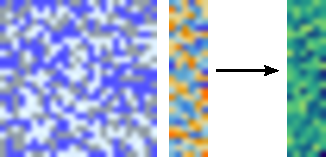
\includegraphics[scale=.75]{randprojmethodillust}}
\vskip2em

\centerline{
\begin{overpic}[scale=.75]{randprojmethod2illust}
 \put(3,-13){\fcolorbox{gray}{white}{$\matQ$}}
 \put(40,30){\fcolorbox{gray}{white}{$\matQ\transp$}}
 \put(105,-13){\fcolorbox{gray}{white}{$\matA$}}
 \put(180,-13){\fcolorbox{gray}{white}{$\matP_{\matA\matS} \matA$}}
\end{overpic}
}
%\centerline{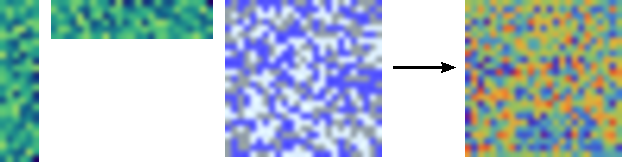
\includegraphics[scale=.75]{randprojmethod2illust}}
% round sphere -> ellipsoid animated illustration 

\end{frame}


% \begin{frame}{Optimal rank-$k$ approximation}
% Fix $\matA \in \R^{m \times n}$ with $m \geq n.$
% 
% The most accurate rank-$k$ approximation in the spectral and Frobenius norms
% \[
%  \matA_k = \underset{%
%                \substack{%
%                  \matM \in \R^{m \times n} \\ 
%                  \operatorname{rank}(\tilde{\matA}) \leq k}}%
%            {\operatorname{argmin}}  
%            \|\matA - \matM\|_\xi, \quad \text{ for $\xi \in \{2, \mathrm{F}\}$}.
% \]
% can be computed in $\mathrm{O}(mn^2)$ time via the Singular Value Decomposition (SVD): if\vspace{-1em}
% \[
% \mat{A} = \mat{U} \matSig \mat{V}\transp = \bbordermatrix{%
% &^k \vspace{-0.75ex} & \!\!^{n-k}  \hspace{1ex}\cr
% & \vspace{0.25ex} \mat{U}_1 \hspace{-2ex} & \mat{U}_2 
% }
% \bbordermatrix{%
% & \vspace{-0.75ex} ^k &\!\!^{n-k} \hspace{1ex}\cr
% & \matSig_1 & \cr
% & \vspace{0.5ex} & \matSig_2 
% }
% \left[
% \begin{matrix}
% \mat{V}_1\transp \\
% \mat{V}_2\transp  
% \end{matrix}
% \right]
% \]
% then $\matA_k = \matU_1 \matSig_1 \matV_1\transp.$
% 
% \end{frame}

% \begin{frame}
%  We measure the approximation accuracies relative to those of $\matA_k,$ obtained
%  from a rank-$k$ truncated SVD of $\matA.$
%  
%  \begin{itemize}
%   \item An approximation $\matM$ satisfies a \emph{relative-error bound} if
%            \[
%            \|\matA - \matM\|_\xi \leq (1 + \epsilon) \|\matA - \matA_k\|_\xi 
%            \]
%   for an $\epsilon > 0.$
%   
%   \item It satisfies an \emph{additive-error bound} if 
%            \[
%             \|\matA - \matM\|_\xi \leq \|\matA - \matA_k\|_\xi + \epsilon
%            \]
%   for an $\epsilon > 0.$ In this case, $\epsilon$ is called the \emph{additional error}.
%  \end{itemize}
% 
%  
% \begin{block}{Our objective}
% Find relative- and additive-error bounds for the low-rank approximation
% schemes adhering to the random projection and SPSD sketching methodologies.
% \end{block}
%  
% \end{frame}

\begin{frame}
 
 Our design parameters: 
  \begin{itemize}
   \item $\ell,$ the number of samples ($k \leq \ell \ll \min\{m,n\}$) 
   \item $\matS \in \R^{n \times \ell},$ the random sampling matrix.
  \end{itemize}

 \vspace{1em}
 We approximate $\matA$ with $\matP_{\matA \matS} \matA:$
 
 \begin{enumerate}
  \item Form $\matY = \matA \matS.$
  \item Take the QR decomposition $\matY = \matQ \matR.$
  \item Form the low rank approximation $\matQ (\matQ\transp \matA).$
 \end{enumerate}
Requires only two passes over $\matA.$

 \vspace{1em}
 The quality of the approximation depends on how well the range of the dominant $k$-dimensional left
 singular space of $\matA$ is approximated by the range of $\matY.$
 
 \vspace{1em}
 This methodology was popularized by \refer{Papadimitriou et al. 2000}, \refer{Sarl{\'o}s 2006}, and \refer{Martinsson et al. 2006}.
\end{frame}

\begin{frame}
Three factors determine probability of getting a good approximation:

\begin{itemize}
 \item Spectral decay of $\matA$, e.g. the multiplicative gap $\sigma_{k+1}(\matA)/\sigma_k(\matA).$
 \item Type of randomness used to generate $\mat{S}.$
 \vskip1em
 \centerline{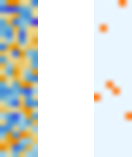
\includegraphics{samplingschemesillust}}
 \vskip1em
 \item Amount of oversampling (as $\ell \rightarrow n, \mat{P}_{\mat{A} \mat{S}} \mat{A} \rightarrow \mat{A}$).
\end{itemize}

\end{frame}

\begin{frame}{Choice of sampling matrix}

Dominant arithmetic cost of forming these low-rank approximations is the matrix multiply $\matA\matS.$
\vspace{1em}

A natural choice for $\matS$ is a matrix of i.i.d. $\mathcal{N}(0,1)$ Gaussians, proposed in \refer{Martinsson et al. 2006}. 
\begin{itemize}
 \item Computation of 
$\matA \matS$ takes $\const{O}(mn\ell)$ time for general $\matA$.
 \item The columns of $\matA$ are well-mixed.
\end{itemize}

\vspace{1em}

\refer{Woolfe et al. 2008} proposed using \emph{structured} random projections.

\begin{itemize}
 \item Computation of $\matA \matS$ takes reduced time $\const{O}(mn \log(\ell)).$
 \item Mixing not as uniform, so potential accuracy loss.
\end{itemize}

\end{frame}

\begin{frame}
 Assume $n$ is a power of $2.$ We consider the case where $\matS$ is a subsampled randomized Hadamard transform (SRHT):
 \[
  \matS = \sqrt{\frac{n}{\ell}} \matD \matH \matR \in \R^{n \times \ell}.
 \]
Here:
\begin{itemize}
 \item  $\matD$ is a diagonal matrix of random signs,
 \item  $\matR$ selects $\ell$ columns at random, and 
 \item $\matH = n^{-1/2} \matH_n \in \R^{n \times n}$ is the normalized Walsh--Hadamard matrix. The matrices $\matH_n$ are
defined recursively by
\[
 \matH_n = \left[
\begin{array}{cc}
  \matH_{n/2} &  \matH_{n/2} \\
  \matH_{n/2} & -\matH_{n/2}
\end{array}\right],
%
\qquad \mbox{with} \qquad
%
\matH_2 = \left[
\begin{array}{cc}
  +1 & +1 \\
  +1 & -1
\end{array}\right].
\]
\end{itemize}

The matrix--matrix product $\matA \matS$ can be computed in time $\mathrm{O}(mn\log\ell).$
\end{frame}


\begin{frame}{Empirical performance}
 
 Let $n = 1024;$ consider the following test matrix in $\R^{(n+1)\times n}$:
\[ \matA = [100 \vec{e}_1 + \vec{e}_2, 100 \vec{e}_1
 + \vec{e}_3, \ldots, 100 \vec{e}_1 + \vec{e}_{n+1}], \]
where $\vec{e}_i \in \R^{n+1}$ are the standard basis vectors.

\vspace{1em}
$\matA$ is approximately rank-one, and all its columns are biased toward the dominant left singular-vector $\vec{e}_1.$
\end{frame}

\begin{frame}
 \centerline{%
 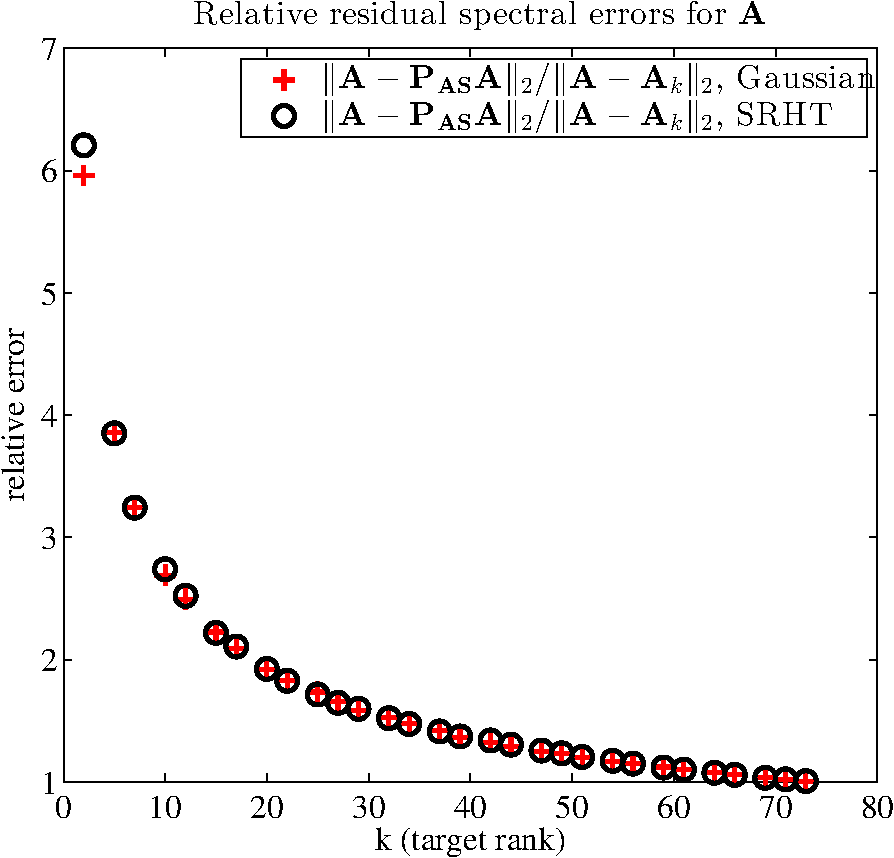
\includegraphics[width=2.2in, keepaspectratio=true]{experimentA-residual-spectral.pdf}%
 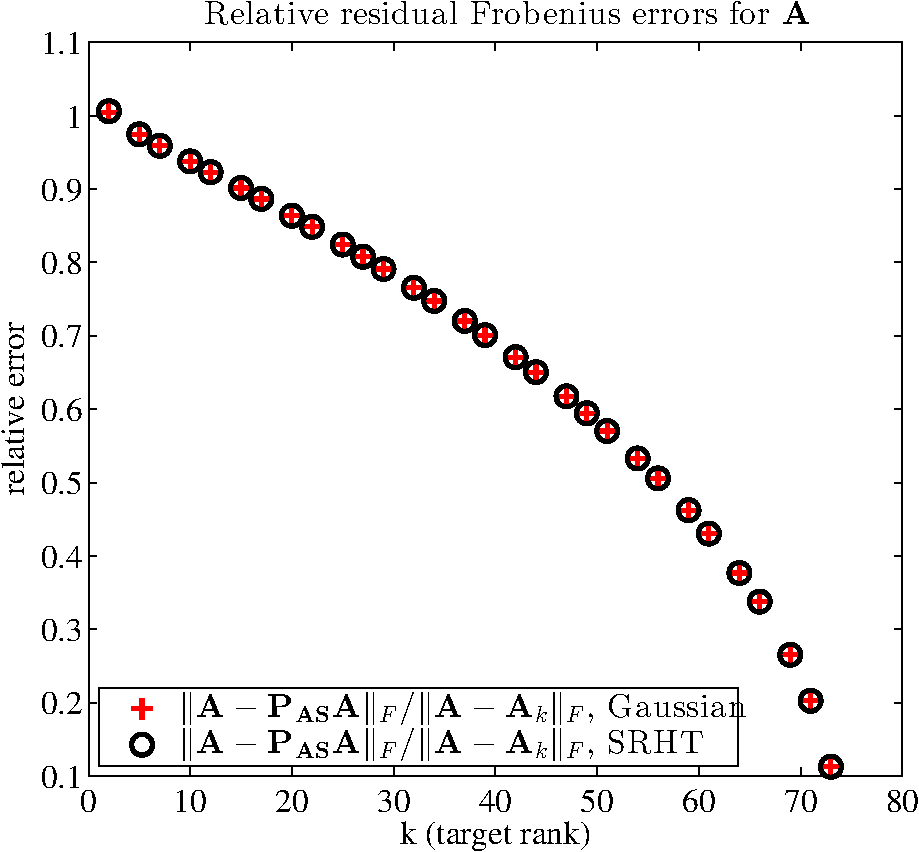
\includegraphics[width=2.2in, keepaspectratio=true]{experimentA-residual-frobenius.pdf}}
 \vspace{1em}
  Each point is the average of the errors observed over 30 trials,
 where each approximation was constructed using $\ell = \lceil 2 k \log n \rceil.$
 
\end{frame}

\begin{frame}

 Let $n = 1024;$ consider the diagonal matrix $\matB \in \R^{n \times n}$ with 
 entries $(\matB)_{ii} = 100(1 - (i-1)/n).$
 \[
  \matB = \left[ 
          \begin{matrix} 100 &  0     & 0 & \ldots \\
                          0  & 99.902 & 0 & \ldots \\
                          0  & 0      & \ddots & \ldots \\
                          0  & \ldots & 0 & 0.098 
          \end{matrix}
          \right]
 \]

  $\matB$ is full-rank, has slowly decaying spectrum, and only $k$ columns of $\matB$
  provide any information on the dominant $k$-dimensional left singular space of $\matB.$
\end{frame}
 
\begin{frame}
\centerline{%
 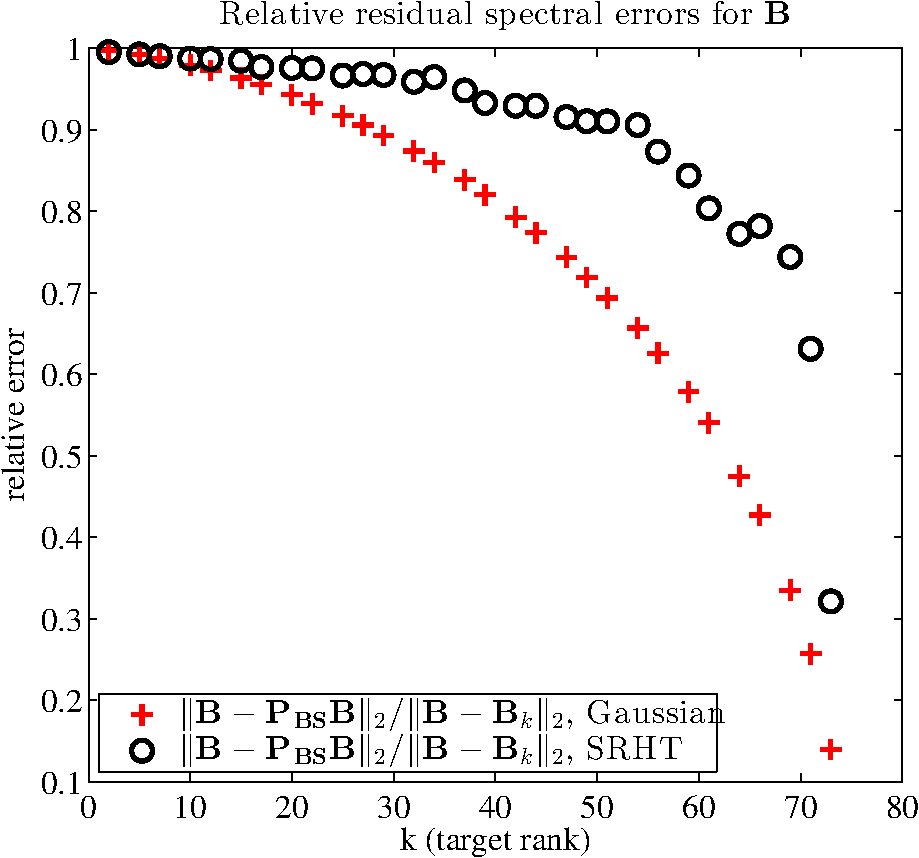
\includegraphics[width=2.2in, keepaspectratio=true]{experimentB-residual-spectral.pdf}%
 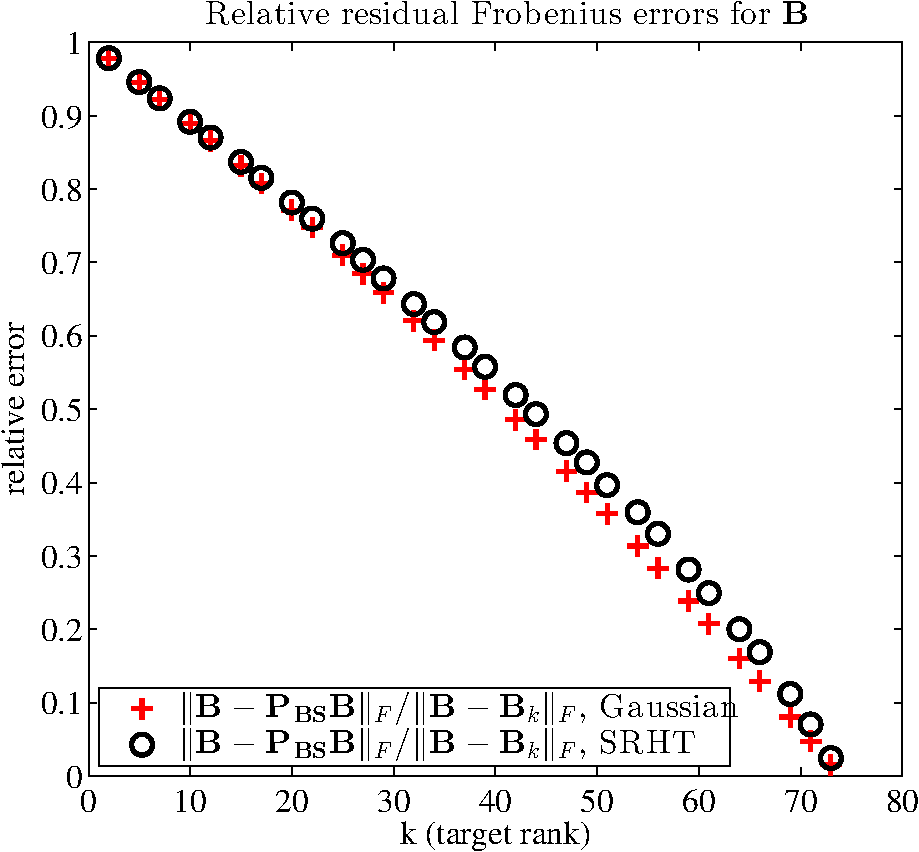
\includegraphics[width=2.2in, keepaspectratio=true]{experimentB-residual-frobenius.pdf}}
 \vspace{1em}
 Each point is the average of the errors observed over 30 trials,
 where each approximation was constructed using $\ell = \lceil 2 k \log n \rceil.$
\end{frame}

\begin{frame}
  
 Consider $\matC = \matU \matB \matV\transp,$ where $\matU$ and $\matV$
 are obtained by taking the SVD of an $n \times n$ matrix of i.i.d. $\mathcal{N}(0,1)$ random variables,
 $\matG = \matU \matSig \matV\transp.$
 
\[
 \matC = \matU \left[ 
          \begin{matrix} 100 &  0     & 0 & \ldots \\
                          0  & 99.902 & 0 & \ldots \\
                          0  & 0      & \ddots & \ldots \\
                          0  & \ldots & 0 & 0.098 
          \end{matrix}
          \right] \matV\transp
\]

 $\matC$ is also full-rank and has slowly decaying spectrum, but every column of $\matC$ contains
 information on every singular space of $\matC.$
\
\end{frame}

 \begin{frame}
\centerline{%
 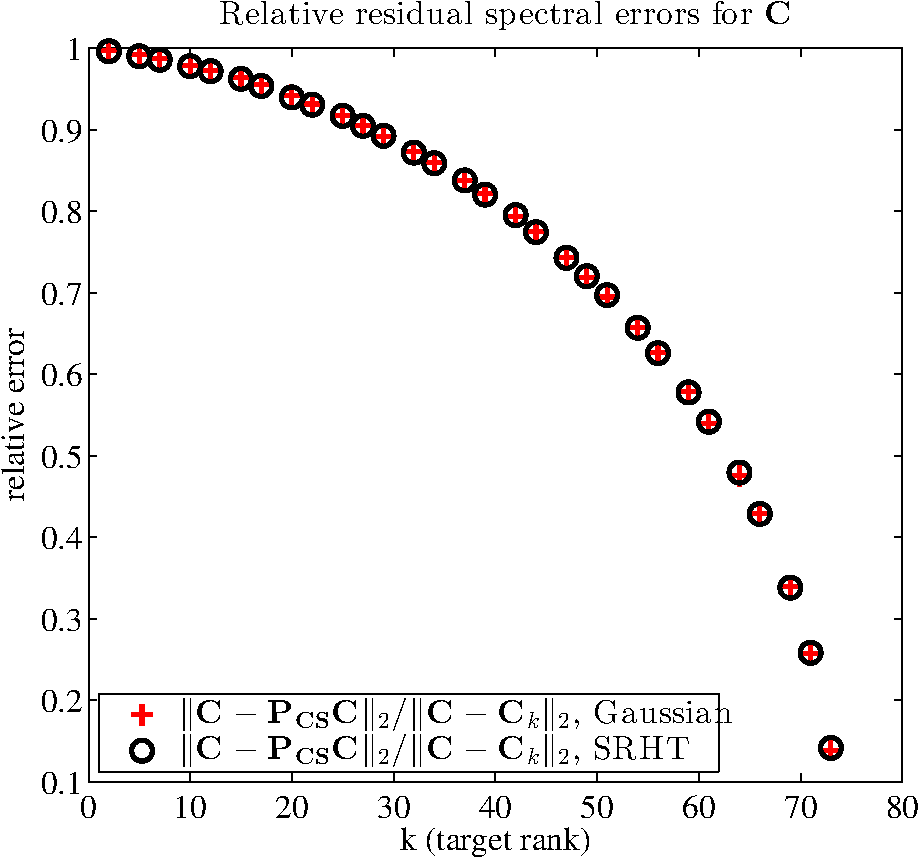
\includegraphics[width=2.2in, keepaspectratio=true]{experimentC-residual-spectral.pdf}%
 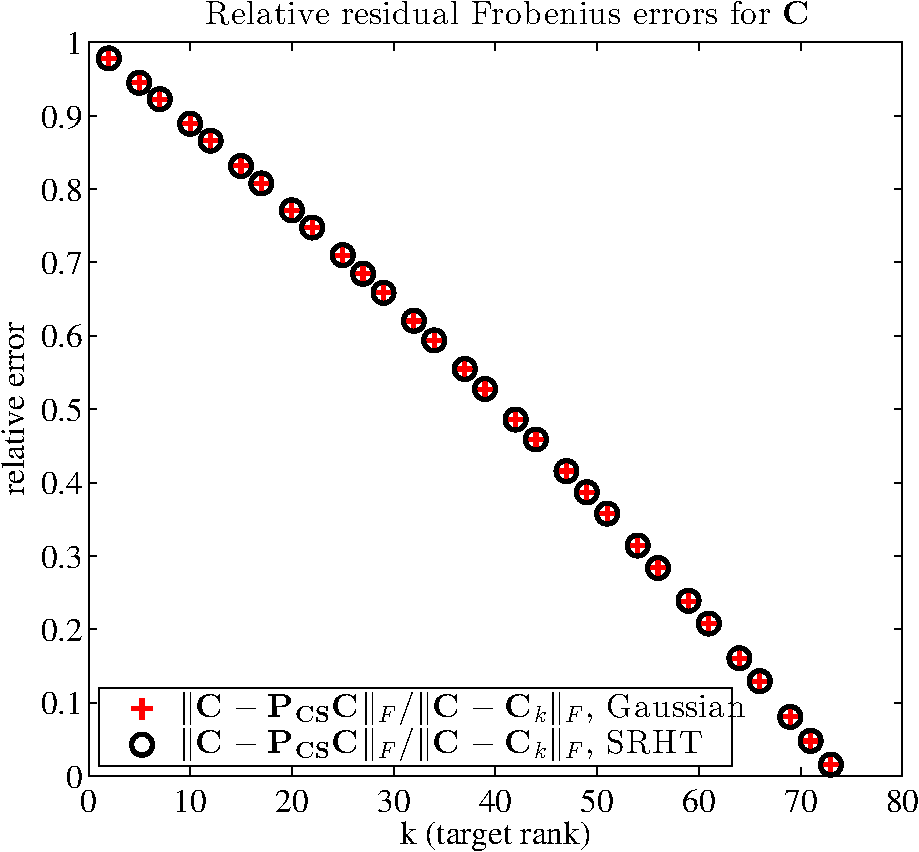
\includegraphics[width=2.2in, keepaspectratio=true]{experimentC-residual-frobenius.pdf}}
 \vspace{1em}
 Each point is the average of the errors observed over 30 trials,
 where each approximation was constructed using $\ell = \lceil 2 k \log n \rceil.$
 \end{frame}

 \begin{frame}
  Observations:
  \begin{enumerate}
   \item When $\matA$ is approximately low-rank, the SRHT and Gaussian low-rank approximations exhibit
   about the same accuracy.
   \item When $\matA$ is full rank the structures of the singular spaces are important. 
   \begin{itemize} 
   \item If the singular
   vectors are ``flat'', then SRHT and Gaussian approximations have comparable accuracy. 
   \item If the singular
   vectors are axis-aligned, then Gaussian approximations outperform SRHT approximations.
   \end{itemize}
   \item Empirically, $\ell = \Omega(k \log n)$ seems to ensure SRHT approximations achieve relative-error bounds.
  \end{enumerate}

 \end{frame}
 
 \begin{frame}{Prior work}

 Similar randomized orthogonal projection schemes:
 \begin{itemize}
  \item \refer{Woolfe et al. 2008}: if $\ell = \const{O}(k^2),$ then 
   \[
     \|\matA - \tilde{\matA}\|_2 = \sqrt{\max\{m,n\}} \|\matA - \matA_k\|_2
   \]
  \item \refer{Nguyen et al. 2009}: if $\ell = \const{O}(\varepsilon^{-1} k \log k),$ then
  \begin{align*}
   \|\matA - \tilde{\matA}\|_2 & \leq (2 + \sqrt{n/\ell}) \|\matA - \matA_k\|_2 \\
   \|\matA - \tilde{\matA}\|_\rf & \leq (1 + \epsilon) \|\matA - \matA_k\|_\rf
  \end{align*}
 \end{itemize}

 Exactly the same SRHT scheme:
 \begin{itemize}
  \item \refer{Halko et al. 2011}: if $\ell = \const{O}(k \log k),$ then for $\xi \in \{2, \rf\},$
  \[ \|\matA - \matP_{\matA \matS}\|_\xi \leq (1 + \sqrt{n/\ell})\|\matA - \matA_k\|_\xi.
  \]
 \end{itemize}

\end{frame}
% 
% \begin{frame}{For comparison}
%  
%  It follows from \refer{Halko et al. 2011} that when $\matS$ is Gaussian and 
%  $\ell = \Omega(\epsilon^{-2} k \log n),$
%  \begin{align*}
%   \|\matA - \matP_{\matA\matS} \matA\|_2 & \leq \left(1 + \frac{\epsilon}{\sqrt{\log n}}\right) \|\matA - \matA_k\|_2
%     + \frac{\epsilon}{\sqrt{k \log n}} \|\matA - \matA_k\|_\rf \\
%   \|\matA - \matP_{\matA\matS} \matA\|_F & \leq \left(1 + \frac{\epsilon}{\sqrt{\log n}}\right) \|\matA - \matA_k\|_F
%     + \frac{\epsilon}{\sqrt{k}} \|\matA - \matA_k\|_2
%  \end{align*}
%  simultaneously with probability at least $1 - \frac{2}{n}.$
%  \vspace{1em}
%  
%  We managed to tighten the gap between the prior bounds for SRHT sampling and this result for Gaussian sampling.
% \end{frame}

\begin{frame}{Improved Error Bounds}
 \begin{block}{\refer{Boutsidis and G. 2012}}
  If $k = \Omega(\log n)$ and $\ell = \Omega( \epsilon^{-2} k \log n ),$ then
  \begin{align*}
      \|\matA - \matP_{\matA\matS} \matA\|_2 & \leq 
       (4 + \epsilon )\cdot \|\matA - \matA_k\|_2 + \frac{\epsilon}{\sqrt{k}} \|\matA - \matA_k\|_\rf \\
   \|\matA - \matP_{\matA\matS} \matA\|_\rf & \leq (1 + 11\epsilon^2) \|\matA - \matA_k\|_\rf
  \end{align*}
  simultaneously with probability at least $1 - \delta.$
 \end{block}

 This result essentially holds when $\matS$ is any subsampled orthogonal transformation,
 \[
  \matS = \sqrt{\frac{n}{\ell}} \matD \matT \matR,
 \]
 where $\matT$ is an orthogonal transformation matrix with entries on the order of $n^{-1/2}.$
\end{frame}

\begin{frame}{Notation}
\begin{itemize}
 \item Partition the SVD of $\matA:$
\vspace{-1em}
 \[ 
\mat{A} = \mat{U} \matSig \mat{V}\transp = \bbordermatrix{%
&^k \vspace{-0.75ex} & \!\!^{n-k}  \hspace{1ex}\cr
& \vspace{0.25ex} \mat{U}_1 \hspace{-2ex} & \mat{U}_2 
}
\bbordermatrix{%
& \vspace{-0.75ex} ^k &\!\!^{n-k} \hspace{1ex}\cr
& \matSig_1 & \cr
& \vspace{0.5ex} & \matSig_2 
}
\left[
\begin{matrix}
\mat{V}_1\transp \\
\mat{V}_2\transp  
\end{matrix}
\right].
\]
 Note that $\matA_k = \matU_1 \matSig_1 \matV_1\transp.$ 

 \item Define
\[
 \matOmega_1 = \matV_1\transp \matS \quad \text{ and } \matOmega_2 = \matV_2\transp \matS,
\]
to capture the interaction of $\matS$ with the dominant and residual right singular spaces of $\matA.$
\vspace{1em}
\end{itemize}

\end{frame}

\begin{frame}{Proof sketch}

  \begin{block}{\refer{Boutsidis et al. 2011}, \refer{Halko et al. 2011} }
  If $\matOmega_1 = \matV_1\transp \matS$ has full row rank, then
  \[
   \|\matA - \matP_{\matA\matS} \matA\|_\xi^2 \leq \|\matA - \matA_k\|_\xi^2 + \bigbar \matSig_2 \matOmega_2 \matOmega_1^\pinv\bigbar_\xi^2
  \]
  for $\xi \in \{2, \rf\}.$
 \end{block}

 Geometrical interpretation:
 \begin{itemize}
  \item $\matV_1\transp \matS \text{ has full row-rank } \Leftrightarrow \tan(\matV_1, \matS) \neq \infty.$ 
  \item $\bigbar\matOmega_2 \matOmega_1^\pinv\bigbar_2 = \tan(\matV_1, \matS).$
 \end{itemize}

 We bound the additional errors $\bigbar \matSig_2 \matOmega_2 \matOmega_1^\pinv\bigbar_2^2$ and $\bigbar \matSig_2 \matOmega_2 \matOmega_1^\pinv\bigbar_\rf^2$
 when $\matS$ is an SRHT.
 \vspace{0.7em}
 
 The key tool is an extension of a result in \refer{Tropp 2011} to show right multiplication by $\matD\matH$ distributes the energy of the matrix
 evenly over its columns.

\end{frame}

% \begin{frame}{Proof sketch}
% \begin{itemize}
%  \item Bounding $\bigbar \matSig_2 \matOmega_2 \matOmega_1^\pinv\bigbar_2^2$ and $\bigbar \matSig_2 \matOmega_2 \matOmega_1^\pinv\bigbar_\rf^2$
%  reduces to showing that the columns of $\matM \matD \matH$ all have roughly the same norm when $\matM$ is an arbitrary matrix:
%  \[
%   \max_{j=1,\ldots,n} \|(\matM \matD \matH)_{j}\|_2 \leq \frac{\|\matM\|_\rf}{\sqrt{n}} + \frac{t\|\matM\|_2}{\sqrt{n}} 
%  \]
% with high probability. 
%  \item \refer{Tropp 2011} shows this is true when
% $\matM$ has orthonormal rows. The result for arbitrary $\matM$ is a generalization of this argument.
% 
% \end{itemize}
% \end{frame}

 \begin{frame}{SPSD Sketches}
 
 If $\matA$ is a positive semidefinite matrix, one may want to \emph{preserve positivity}. 
 SPSD sketches do so:
  \[
   \mat{A} \approx \mat{C} \mat{W}^\pinv \mat{C}\transp
  \]
  where $\mat{C} = \mat{A} \mat{S}$ and $\mat{W} = \mat{S}\transp \mat{A} \mat{S}.$

Consider, e.g., if $\mat{C}$ corresponds to randomly selected columns of $\mat{A}.$
\centerline{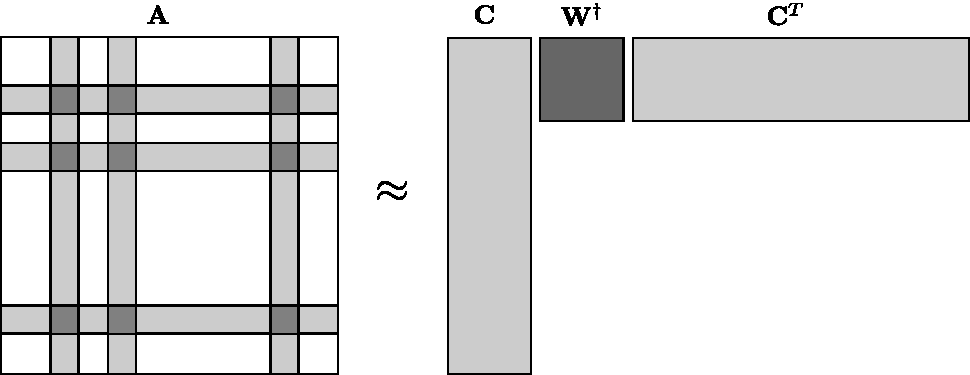
\includegraphics[width=4in,keepaspectratio=true]{nystrom-procedure}}

It takes $\const{O}(\ell^3 + n \ell^2)$ operations to form this approximation.
\end{frame}

\begin{frame}
The class of SPSD sketches is wide. We consider the following specific sketches:
 \begin{itemize}
  \item When $\matS$ selects columns uniformly at random without replacement from $\matA,$ 
   we call $\matM$ a \textcolor{dgreen}{\emph{Nystr\"om extension}}.
  \item When $\matS$ consists of i.i.d. $\mathcal{N}(0,1)$ Gaussians, $\matM$ is a \textcolor{dgreen}{Gaussian sketch}.
  \item When $\matS$ is a subsampled randomized Fourier transform (SRFT), $\matM$ is an \textcolor{dgreen}{SRFT sketch}.
  \item When $\matS$ selects columns from $\matA$ randomly with replacement with probability proportional to their 
   \emph{leverage scores}, $\matM$ is a \textcolor{dgreen}{leverage sketch}.
 \end{itemize}

 SPSD sketches introduced in \refer{G. and Mahoney 2013} as a generalization of Nystr\"om extensions. They require
 one pass over $\matA.$
\end{frame}

% \begin{frame}{Nystr\"om extensions}
% 
% \begin{itemize}
%   \item Introduced in \refer{Williams and Seeger 2001} as a fast way
% of approximating the eigenvectors of large SPSD matrices arising in machine learning.
% 
%  \item Here $\matS$ selects $\ell$ columns uniformly at random from $\matA.$ 
%  
% \centerline{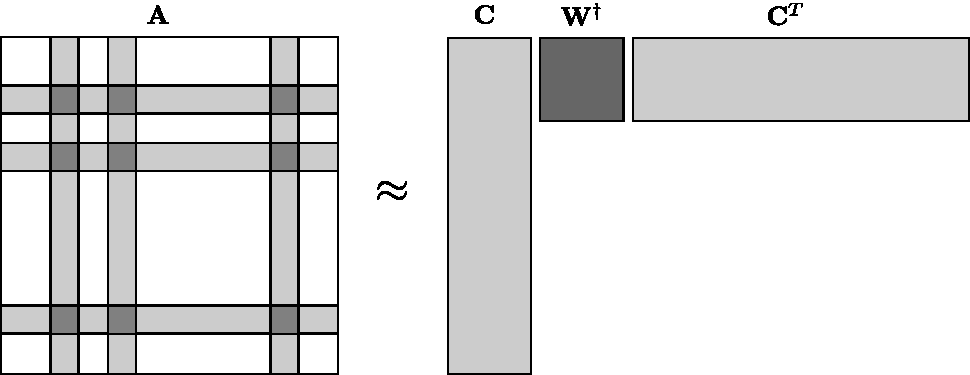
\includegraphics[width=4in,keepaspectratio=true]{nystrom-procedure}}
% 
%  \item It takes $\const{O}(\ell^3 + n \ell^2)$ operations to form this extension (for $p=1$).
% \end{itemize}
% 
% \end{frame}

\begin{frame}{Gaussian and SRFT sketches }
 
  Gaussian and SRFT sketches:
 \begin{itemize}
   \item SRFT sketching suggested in \refer{Chiu and Demanet 2012}
   \item $\matS$ mixes the columns of $\matA$ together before sampling.
   \item Mixing process ensures that no columns are ignored.
   \item Gaussian sketches cost $\const{O}(\ell^3 + n^2 \ell)$ operations to form.
   \item SRFT sketches cost $\const{O}(\ell^3 + n^2 \log \ell)$ operations to form.
   
\end{itemize}
 
\end{frame}


\begin{frame}{Leverage scores}
The statistical leverage scores of the columns of $\mat{A}$ (with respect to rank $k$), are the scaled column norms
of $\matU_1\transp:$
\[
 \left\{ \ell_j := \frac{n}{k} \snorms{(\matU_1\transp)_j}, j=1,\ldots,n \right\}.
\]
\vfill
%\centerline{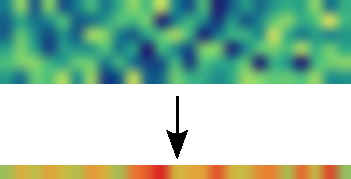
\includegraphics{levscoresillust}}
\centerline{
\begin{overpic}{levscoresillust}
 \put(-25,65){\fcolorbox{gray}{white}{$\matU_1\transp$}}
 \put(-29,0){\fcolorbox{gray}{white}{$\{\ell_j\}$}}
\end{overpic}
}
\vfill

\end{frame}

% \begin{frame}
% Leverage scores expose the dependence of the columns of $\mat{A}$ on $\matU_1.$ 
% \begin{itemize}
%  \item Let $\matA_j$ denote the $j$th column of $\matA$ and
% $\mat{u}_i$ denote the $i$th eigenvector, then
% \[
%  \mat{A}_j = \sum_{i=1}^{n} \lambda_i (\mat{u}_i \mat{u}_i^t)_j = \sum_{i=1}^k \lambda_i (\matU_1)_{ji} \mat{u}_i + \cdots
% \]
% so
% \[
%  \ell_j \propto \snorms{(\matU_1)_j} = \sum_{i=1}^k (\matU_1)_{ji}^2 
% \]
% is a measure of the influence $\matU_1$ has on $\mat{A}_j.$
%  \item We expect that columns with larger leverage scores provide more information on $\matU_1.$
% \end{itemize}
% 
% \end{frame}

\begin{frame}{Leverage sketches}

Leverage sketches:
 \begin{itemize}
 \item The idea of leverage score sampling for forming column-sampling based low-rank approximations due to \refer{Drineas et al. 2008}.
  \item Columns are sampled random from $\matA$ with probability proportional to their leverage scores.
  \item Intuitively, leverage score sampling ensures that no important columns are ignored.
  \item Assuming the leverage scores as given, costs $\const{O}(\ell^3 + n^2 \ell)$ operations to form.
  \item The leverage scores can be approximated.
 \end{itemize}

\end{frame}

\begin{frame}{Empirical Performance}

\centerline{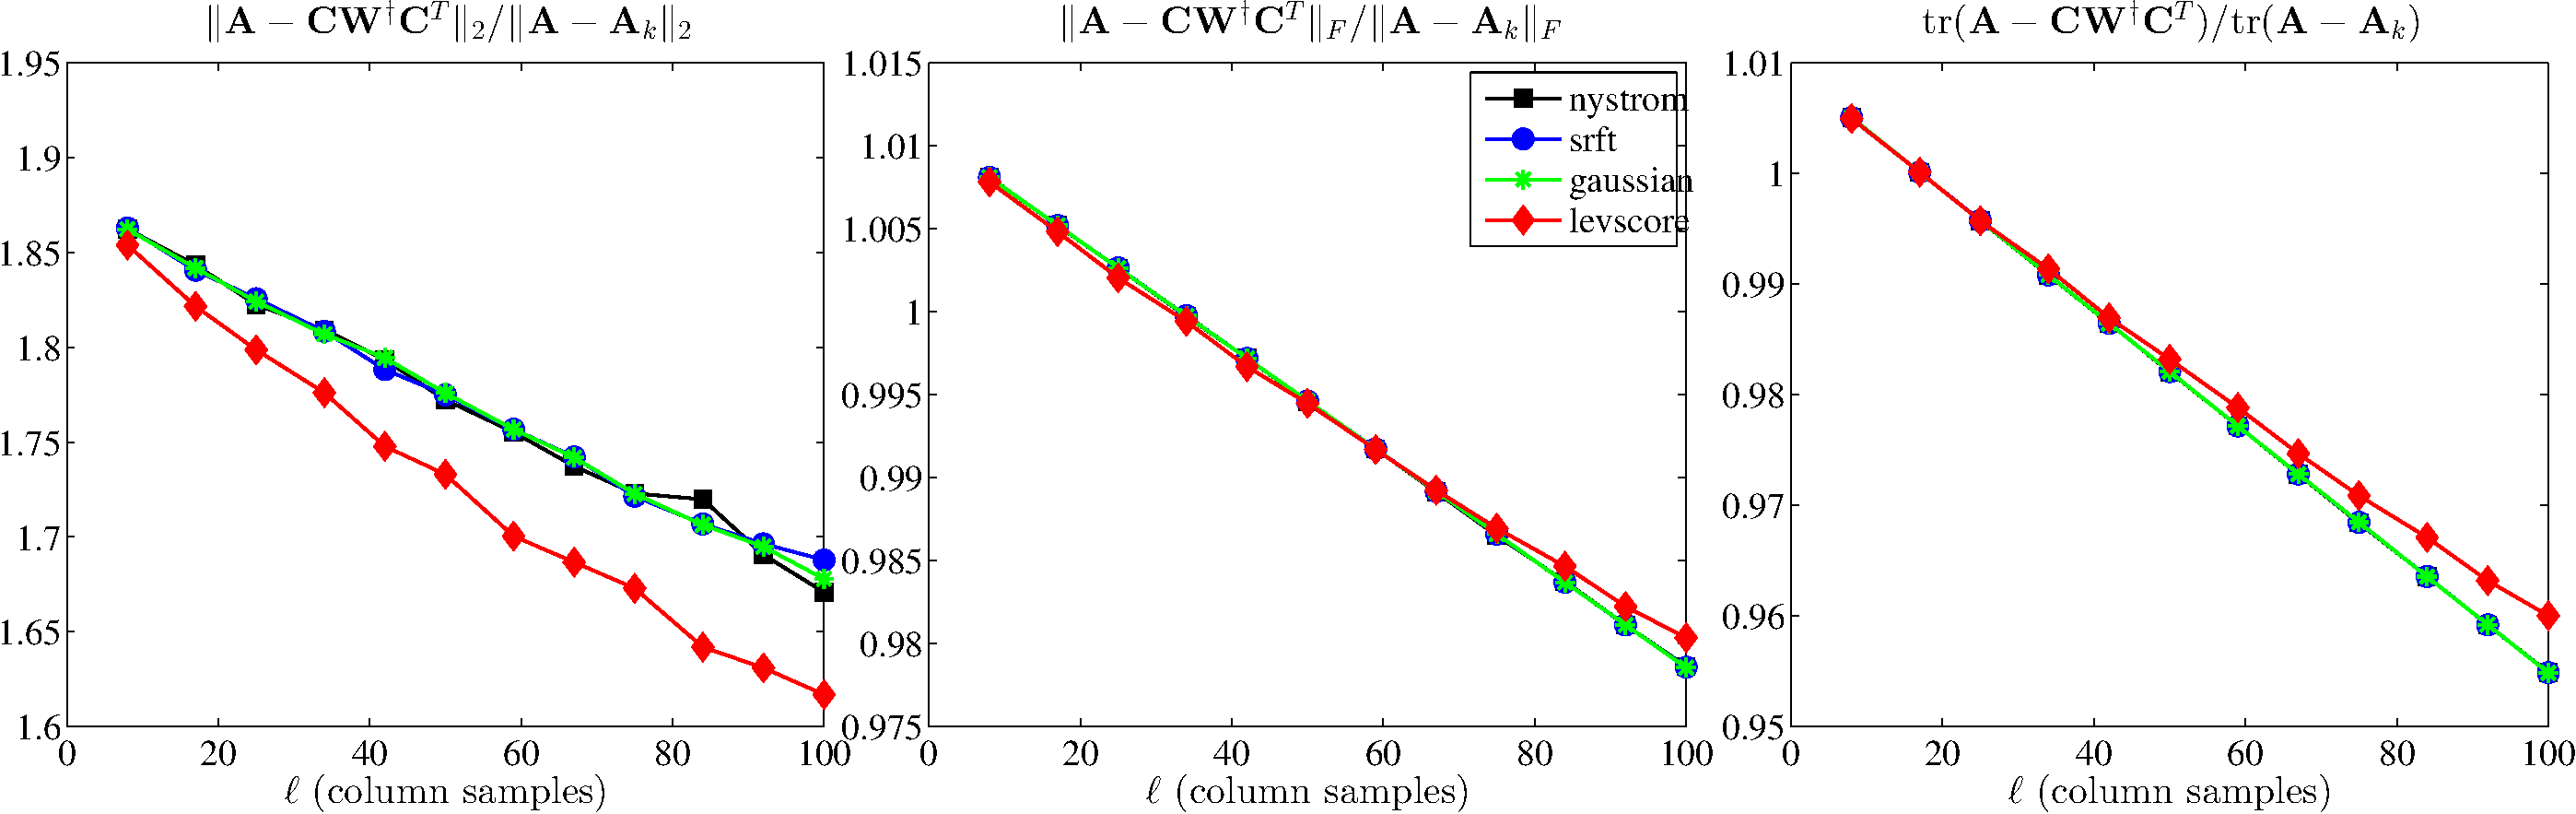
\includegraphics[width=4.7in, keepaspectratio=true]{Dexterrank8exact-methods-nonfixed-rank-errors}}

 Dexter, a $2000 \times 2000$ Gram matrix from the UCI Machine Learning Repository. 
 Target rank $k= 8.$ Each point is the average relative error over 30 trials.
\end{frame}

\begin{frame}

\centerline{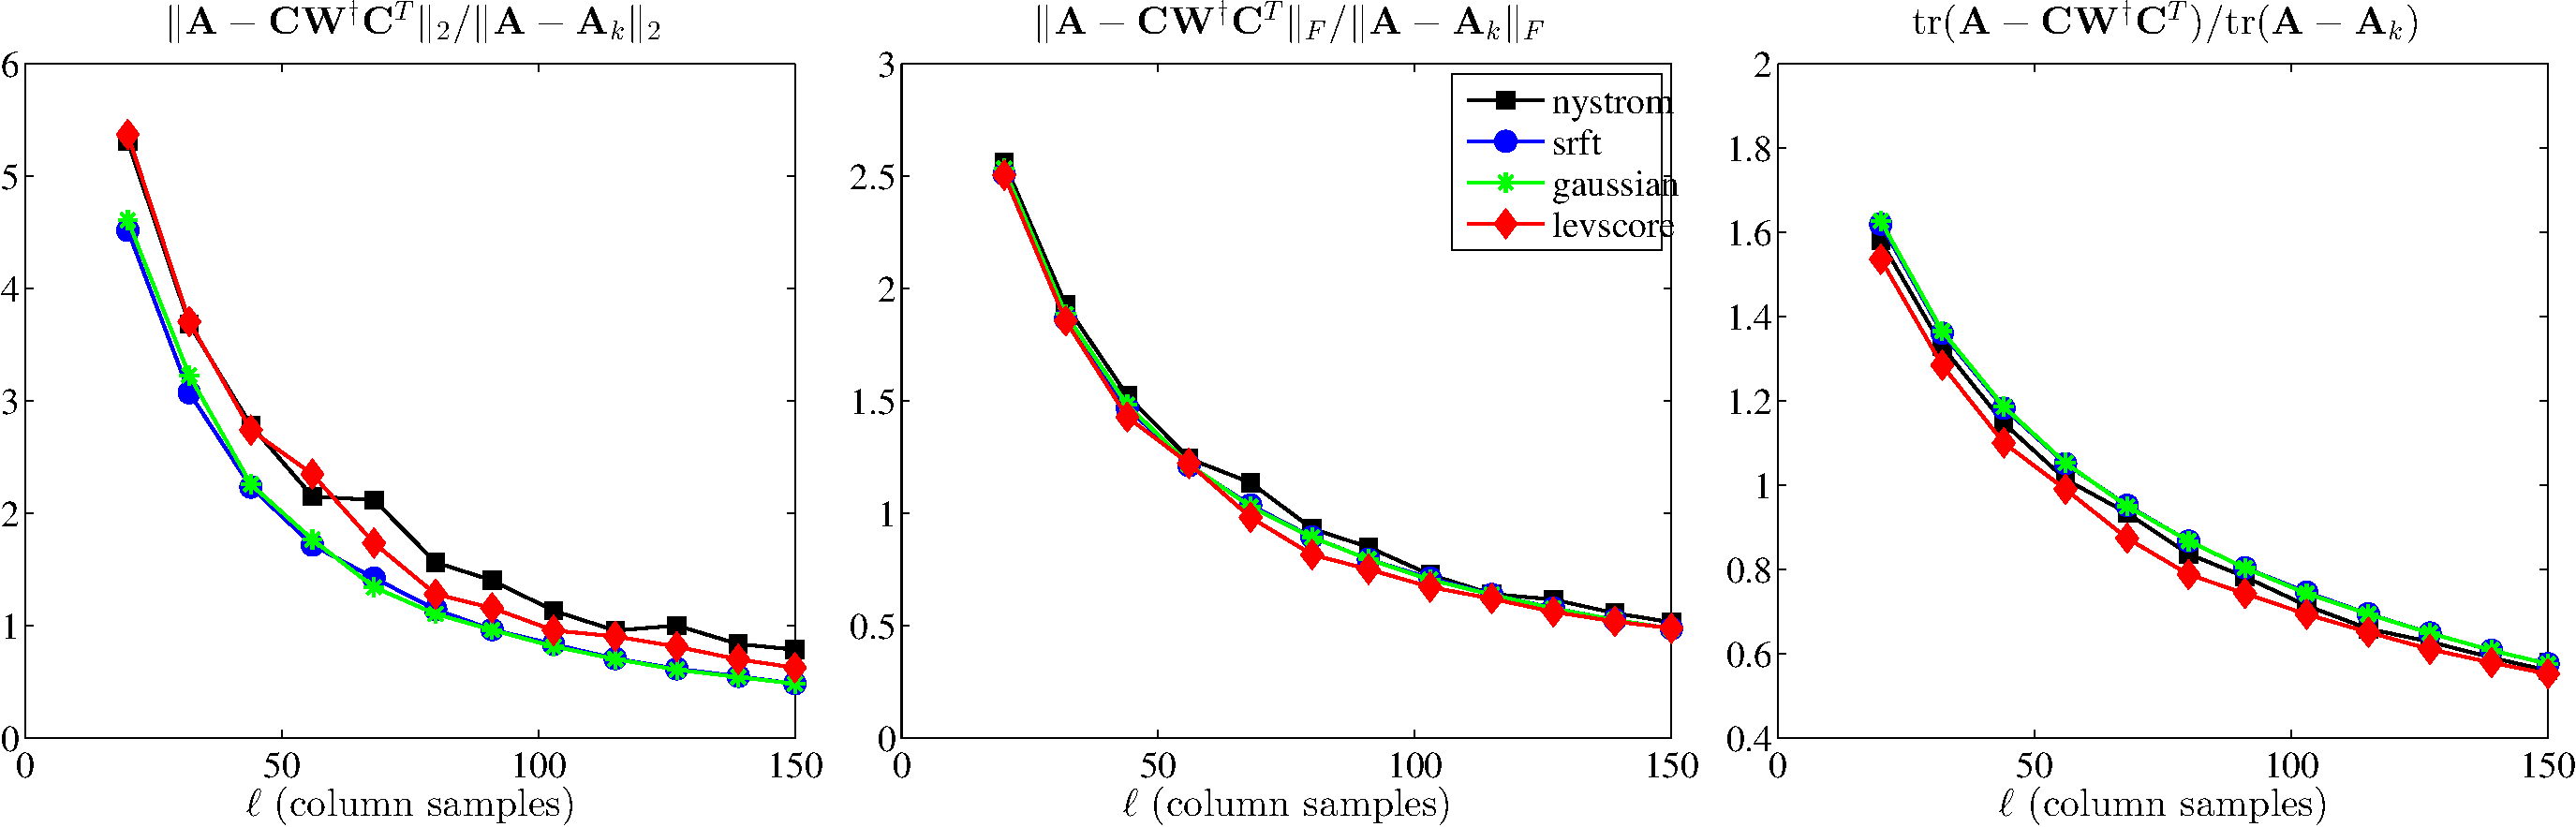
\includegraphics[width=4.7in, keepaspectratio=true]{Abalonesigma1exact-methods-nonfixed-rank-errors}}

 Abalone, a $4898 \times 4898$ Radial Basis Kernel matrix from the UCI Machine Learning Repository. 
 Target rank $k= 20.$ Each point is the average relative error over 30 trials.
\end{frame}

\begin{frame}
 
 \centerline{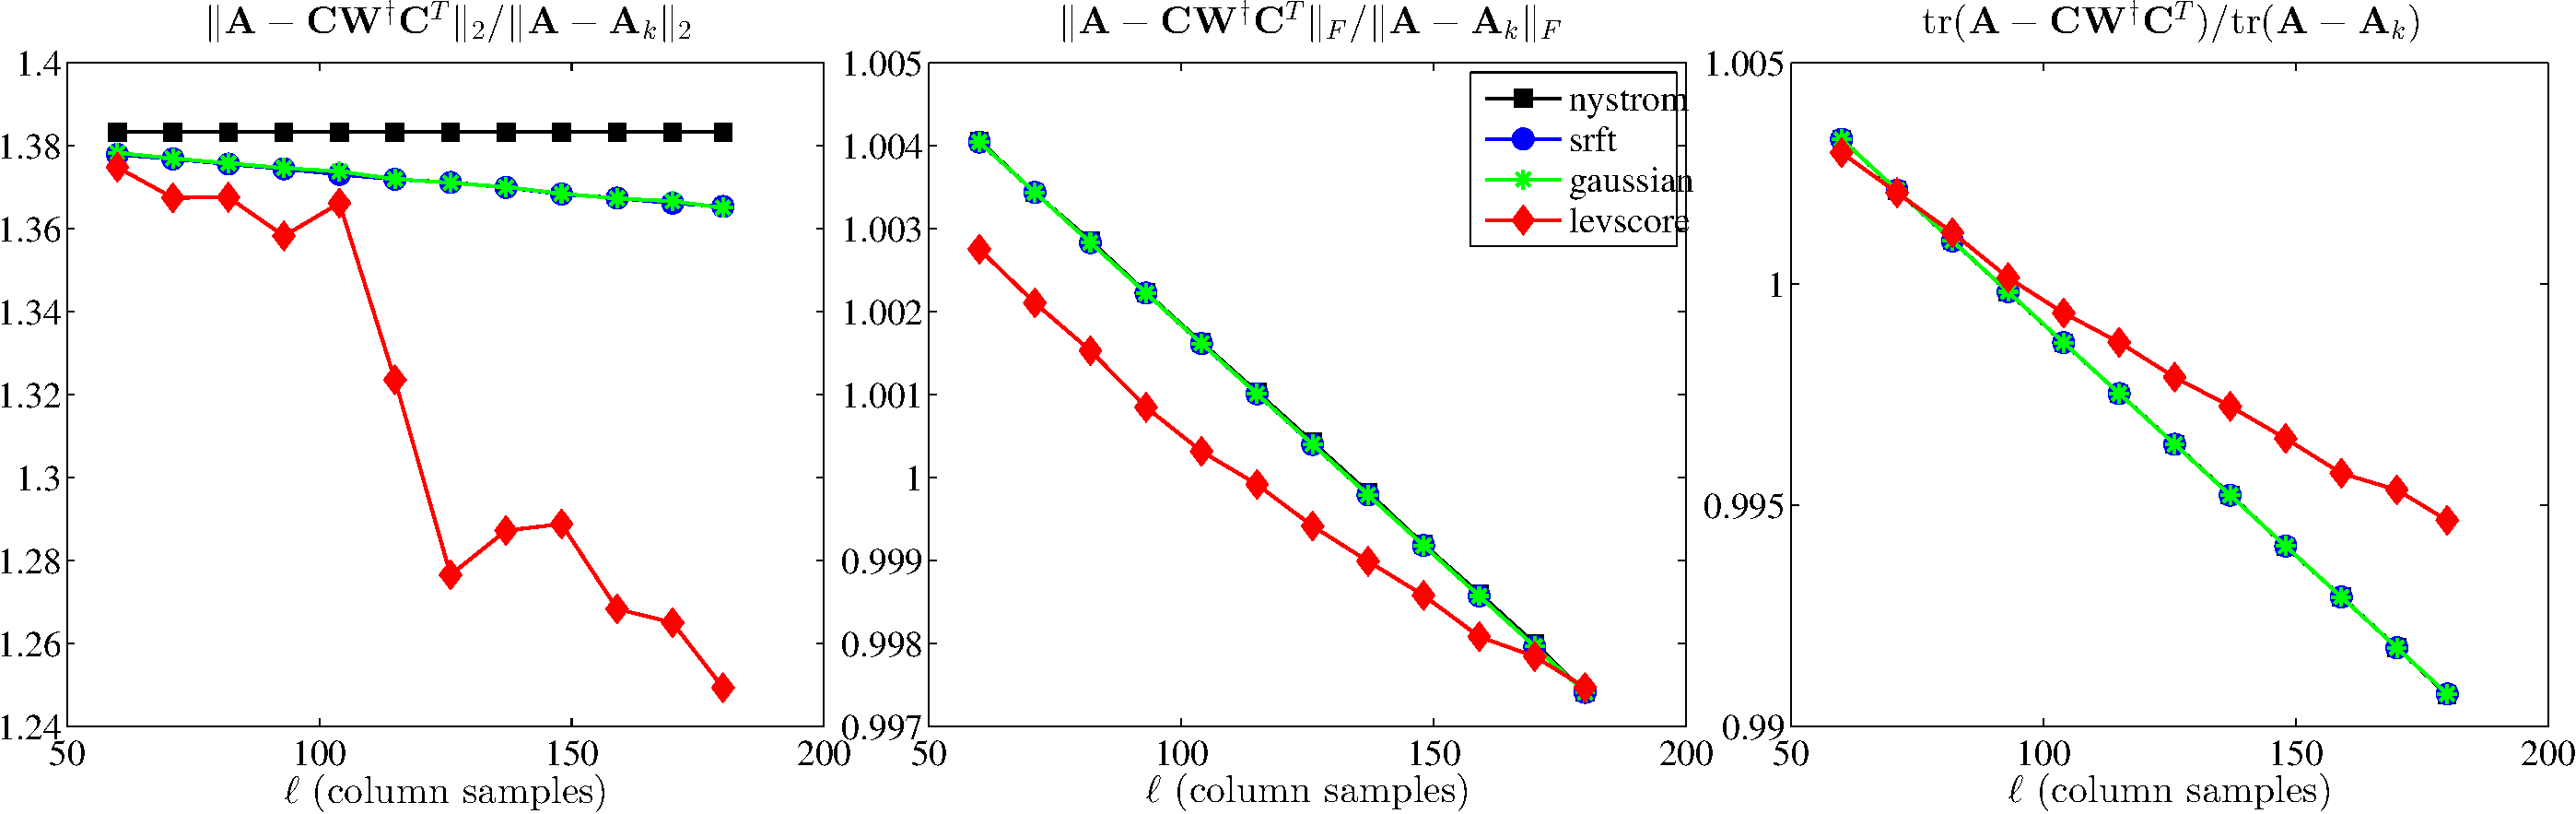
\includegraphics[width=4.5in, keepaspectratio=true]{Enronrank60exact-methods-nonfixed-rank-errors}}
 Enron, a $10K \times 10K$ Graph Laplacian matrix from the Stanford SNAP collection. Target
 rank $k = 60.$ Each point is the average relative error over 30 trials.
\end{frame}

\begin{frame}
Observations:
\begin{itemize}
 \item The leverage sketches are often the most accurate.
 \item The relative trace-norm errors are all smaller than the relative Frobenius-norm errors, which are in turn 
 smaller than the relative spectral-norm errors.
 \item The sketches are more distinguished by their behavior in the spectral norm than the Frobenius or trace norms
\end{itemize}

\end{frame}


\begin{frame}{Prior work}

\centerline{\scriptsize
\begin{tabular}{|l|l|c|}
\hline
Source, sketch & $\ell$ & $\|\matA - \matC\matW^\pinv\matC\transp\|_2$\\
\hline 
\refer{Drineas and Mahoney 2005},          column-sampling & $\Omega(\epsilon^{-4} k)$ & $\|\matA - \matA_k\|_2 + \epsilon \sum_{i=1}^n A_{ii}^2$ \\
\refer{Talwalkar and Rostamizadeh 2010},   Nystr\"om extension        & $\Omega(\mu k \log k)$    & 0, if $\rank(\matA) = k$ \\
\refer{Kwok et al. 2012},                  Nystr\"om extension        & $\Omega(1)$               & $\|\matA - \matA_k\|_2 + n/\sqrt{\ell} \|\matA\|_2$ \\
\refer{Chiu and Demanet 2012},             Nystr\"om extension        & $\Omega(\mu k \log n)$    & $(1 + n/\ell) \|\matA - \matA_k\|_2$ \\
\refer{Chiu and Demanet 2012},             SRFT sketch                & $\Omega(k \log^2 n)$      & $(1 + n/\ell) \|\matA - \matA_k\|_2$ \\
\hline
\end{tabular}
}
\vspace{1em}

\begin{itemize}
 \item Here $\mu \in [1, \frac{n}{k}]$ is the ``coherence'' of the matrix.
 \item The estimated additional error in \refer{Drineas and Mahoney 2005} can be on the order of $\epsilon \tr(\matA).$
 \item The \refer{Talwalkar and Rostamizadeh 2010} exact recovery result requires $\matA$ to be exactly low-rank.
 \item The \refer{Chiu and Demanet 2012} results require $\Omega(k \log n)$ samples as opposed to $\Omega(k \log k).$
       The factor $n/\ell$ is optimal in the Nystr\"om bound, but unnecessary in the SRFT bound.
\end{itemize}

\refer{G. and Mahoney 2013} provides a framework for deriving \emph{significantly} improved error bounds.
\end{frame}

\begin{frame}{Structural error bounds for SPSD sketches}
 Recall the partitioned eigendecomposition of $\mat{A}:$
  \[ \mat{A} = \matU \matSig \matU\transp = [\mat{U}_1 \ \ \mat{U}_2] 
  \left[\begin{matrix} \matSig_1 & \\ & \matSig_2 \end{matrix} \right] 
  [\mat{U}_1 \ \ \mat{U}_2]\transp
  \]
  and that
 \[
  \matOmega_1 = \matU_1\transp \matS \quad \text{ and } \matOmega_2 = \matU_2\transp \matS
 \]
 capture the interactions of the sketching matrices with the dominant and residual eigenspaces of $\matA.$
 \vspace{1em}
 
 If $\matS$ has orthonormal columns, then
 \[
  \bigbar\matOmega_2 \matOmega_1^\pinv\bigbar_2 = \tan(\matS, \matU_1).
 \]

\end{frame}

\begin{frame}
 Our error bounds for SPSD sketches follow from the key observation that 
 \begin{block}{SPSD sketches approximate $\matA^{1/2}$, \refer{G. 2011}}
  \[
   \matC\matW^\pinv \matC\transp = (\matA^{1/2} \matP_{\matA^{1/2} \matS}) (\matP_{\matA^{1/2} \matS} \matA^{1/2}).
  \]
 \end{block}
 Thus the errors of SPSD sketches satisfy
 \[
  \|\mat{A} - \mat{C}\mat{W}^\pinv \mat{C}\transp\|_\xi =
   \|\mat{A} - \matA^{1/2} \mat{P}_{\mat{A}^{1/2} \mat{S}} \mat{A}^{1/2}\|_\xi
 \]
 for $\xi \in \{2, \rf, \text{tr}\}.$
 \vspace{0.7em}
 
 We extend the framework provided in \refer{Halko et al. 2011} for projection-based low-rank approximations
 to find \emph{deterministic} error bounds 
 for SPSD sketches.
\end{frame}

% \begin{frame}{Deterministic spectral-norm error bound}
% 
% Since $\|\matM \matM\transp\|_2 = \|\matM\|_2^2,$ we have
% \begin{align*}
%  \|\mat{A} - \mat{C}\mat{W}^\pinv \mat{C}\transp\|_2 & = 
%  \|\mat{A}^{1/2}(\mat{I} - \mat{P}_{\mat{A}^{p-1/2} \mat{S}} ) \mat{A}^{1/2}\|_2 \\
%  & = \|(\matI - \matP_{\matA^{p-1/2} \mat{S}}) \matA^{1/2}\|_2^2,
% \end{align*}
% A result of \refer{Halko et al. 2011}
% can be used to bound the right hand side quantity. This yields the result
% \begin{block}{Deterministic spectral-norm error bound, \refer{G. and Mahoney 2013}}
% \[
%  \|\matA - \matC \matW^\pinv \matC\transp\|_2 \leq \|\matSig_2\|_2 + \|\matSig_2^{p-1/2} \matOmega_2 \matOmega_1^\pinv\|_2^{2/(2p-1)}.
% \]
% \end{block}
% 
% \end{frame}
% 
% \begin{frame}{Deterministic Frobenius- and trace-norm error bounds}
% 
%  We need to estimate 
%  \[
%   \|\matA - \matC\matW^\pinv \matC\transp\|_\xi = \bigbar\mat{A}^{1/2}(\matI - \mat{P}_{\matA^{p-1/2} \mat{S}} ) \mat{A}^{1/2}\bigbar_\xi
%  \]
% more carefully when $\xi \in \{\rf, \text{tr}\}.$ We extend the argument of (Halko et al. 2011).
% 
% \begin{enumerate}
%  \item Find a \emph{simple} projection $\matM$ satisfying 
%  \[
%  \bigbar\mat{A}^{1/2}(\matI - \mat{P}_{\matA^{p-1/2} \mat{S}} ) \mat{A}^{1/2}\bigbar_\xi \leq 
%  \bigbar \matSig^{1/2}\matM \matSig^{1/2} \bigbar_\xi
% \]
% for $\xi \in \{\rf, \text{tr}\}.$
%  
% \end{enumerate}
% \end{frame}
% 
% \begin{frame}
% \begin{enumerate}
%  \setcounter{enumi}{1}
% 
%  \item Partition
%  \[
%   \matM = \left[ \begin{matrix} \matM_1 & \matM_2 \\ \matM_2\transp & \matM_3 \end{matrix} \right].
%  \]
%  \item Observe that 
%   \[
%   \tr(\matSig^{1/2}\matM \matSig^{1/2} ) = \tr(\matSig_1^{1/2} \matM_1 \matSig_1^{1/2}) + 
%   \tr(\matSig_2^{1/2} \matM_3 \matSig_2^{1/2})
%  \]
%  and
%  \begin{multline*}
%   \bigbar\matSig^{1/2}\matM \matSig^{1/2} \bigbar_\rf^2 = \bigbar\matSig_1^{1/2} \matM_1 \matSig_1^{1/2} \bigbar_\rf^2 + \\
%   2 \bigbar \matSig_1^{1/2} \matM_2 \matSig_2^{1/2} \bigbar_\rf^2 + \bigbar \matSig_2^{1/2} \matM_3 \matSig_2^{1/2} \bigbar_\rf^2.
%  \end{multline*}
% 
%  \end{enumerate}
% 
%  Careful estimate of these terms yields our deterministic bounds.
% \end{frame}
% 
% 
% \begin{frame}
% Let $\gamma = \lambda_{k+1}(\matA)/\lambda_k(\matA)$ denote the multiplicative eigengap.
% \begin{block}{Deterministic Frobenius-norm error bound \refer{G. and Mahoney 2013}}
%  \begin{multline*}
% \|\matA - \matC \matW^\pinv \matC\transp\|_\rf \leq \|\matSig_2\|_F + 
% \gamma^{p-1} \|\matSig_2^{1/2} \matOmega_2 \matOmega_1^\pinv\|_2 \cdot \\
%  \left(\sqrt{2 \tr(\matSig_2)} + \gamma^{p-1} \|\matSig_2^{1/2} \matOmega_2 \matOmega_1^\pinv\|_\rf \right).
% \end{multline*}
% \end{block}
% 
% \begin{block}{Deterministic trace-norm error bound, (G. and Mahoney 2013)}
% \[ \tr(\matA - \matC \matW^\pinv \matC\transp) \leq \tr(\matSig_2) + 
%  \gamma^{2(p-1)} \bigbar \matSig_2^{1/2} \matOmega_2 \matOmega_1^\pinv \bigbar_\rf^2
% \]
% \end{block}
% 
% \end{frame}

\begin{frame} 
 Simplified versions of these bounds:
 \begin{block}{\refer{G. and Mahoney, 2013}}
 If $\matOmega_1 = \matU_1\transp \matS$ has full row rank, then
 \begin{align*}
 \|\matA - \matC \matW^\pinv \matC\transp\|_2 & \leq \left(1 + \bigbar\matOmega_2 \matOmega_1^\pinv\bigbar_2^2\right) \|\matA - \matA_k\|_2 , \\
 \|\matA - \matC \matW^\pinv \matC\transp\|_\rf & \leq \|\matA - \matA_k\|_\rf + 2\sqrt{2} 
 \bigbar {\matOmega_2 \matOmega_1^\pinv} \bigbar_2^2 \cdot \tr(\matA - \matA_k), \text{ and } \\
 \tr(\matA - \matC \matW^\pinv \matC\transp) & \leq 
  \left(1+ \bigbar { \matOmega_2 \matOmega_1^\pinv} \bigbar_2^2 \right) \cdot \tr(\matA - \matA_k)
 \end{align*}
 \end{block}
 
\begin{itemize}
 \item The randomness of $\matS$ enters only through the sketching interaction matrix  ${\matOmega_2 \matOmega_1^\pinv}.$
 \item The spectral-norm and trace-norm additional errors of sketches are proportional to the optimal errors.
 \item The Frobenius-norm additional errors of sketches are proportional to the optimal trace-norm errors.
\end{itemize}

\end{frame}

 \begin{frame}{Spectral error bounds}
  \begin{block}{Leverage sketches}
  If $\ell = \Omega(\epsilon^{-1} k \log(k/\delta))$, then 
  \[
   \|\matA - \matC \matW \matC\transp\|_2 \leq \|\matA - \matA_k\|_2 + \epsilon \tr(\matA - \matA_k)
  \]
  with probability at least $1 - \delta - 0.4.$
 \end{block}
 
 \begin{block}{SRFT sketches}
   If $k = \Omega(\log n)$ and $\ell = \Omega(\epsilon^{-2}k \log(n/\delta))$, then
   \[
  \|\matA - \matC \matW \matC\transp\|_2 \leq \left( 5 + \frac{\epsilon}{\sqrt{k}}\right) \|\matA - \matA_k\|_2 
   + \frac{\epsilon^2}{k} \tr(\matA - \matA_k)
  \]
  with probability at least $1 - \delta.$
 \end{block}

\end{frame}

\begin{frame}

 \begin{block}{Gaussian sketches}
  If $\ell = \Omega((1 + \epsilon^{-1}) k),$ then
  \[
   \|\matA - \matC \matW \matC\transp\|_2 \leq (1 + \epsilon) \|\matA - \matA_k\|_2 + \frac{\epsilon}{k}\tr(\matA - \matA_k)
  \]
  with probability at least $1 - 2k^{-1} - 4\e^{-k\epsilon^{-1}}.$
  \end{block}
  
\end{frame}

%  \begin{frame}{Error bounds for leverage sketches}
%   \begin{block}{\refer{G. and Mahoney 2013}}
%   If $\ell \geq 6400 \epsilon^{-1} k \log(k/\delta)$ where $\epsilon \in (0,1)$ and $\delta \in (0,1),$ then 
%   \begin{align*}
%    \|\matA - \matC \matW \matC\transp\|_2 & \leq \|\matA - \matA_k\|_2 + (\epsilon \tr((\matA - \matA_k)^{2p-1}))^{1/(2p-1)} \\
%    \|\matA - \matC \matW \matC\transp\|_\rf & \leq \|\matA - \matA_k\|_\rf + \sqrt{\epsilon} \gamma^{p-1} \tr(\matA - \matA_k) \\
%    \tr(\matA - \matC \matW^\pinv \matC\transp) & \leq (1 + \epsilon \gamma^{2p-2}) \tr(\matA - \matA_k)
%   \end{align*}
%   simultaneously, with probability at least $1 - 6 \delta - 0.6.$
%  \end{block}
%  
%  \begin{itemize}
%   \item Follows from the deterministic bounds and the analysis of $\bigbar \matSig_2^{1/2} \matOmega_2 \matOmega_1^\pinv\bigbar_\rf$ when $\matS$
%    corresponds to leverage sketching given in (Mackey et al. 2012).
%   \item The large constant 6400 and the failure probability (bounded away from zero) are artifacts of the analysis.
%  \end{itemize}
%  \end{frame}
 
%  \begin{frame}{Error bounds for SRFT sketches}
%   \begin{block}{(G. and Mahoney, 2013)}
%    If $\ell \geq 24 \epsilon^{-1} [\sqrt{k} + \sqrt{8\log(8n/\delta)}]^2 \log(8k/\delta),$ where $\epsilon \in (0,1/3)$ and
%    $\delta \in (0,1),$ then
%    \begin{align*}
%   \|\matA - \matC \matW \matC\transp\|_2 & \leq \|\matA - \matA_k\|_2 \\
%   & + 
%   \const{O}\left(\frac{\log(n/\delta)}{(1- \sqrt{\epsilon}) \ell} \right)^{1/(2p-1)} \tr((\matA - \matA_k)^{2p-1})^{1/(2p-1)} \\
%    \|\matA - \matC \matW \matC\transp\|_\rf & \leq \|\matA - \matA_k\|_\rf + 16 \sqrt{\epsilon} \gamma^{p-1} \tr(\matA - \matA_k) \\
%    \tr(\matA - \matC \matW^\pinv \matC\transp) & \leq (1 + 11 \epsilon \gamma^{2p-2}) \tr(\matA - \matA_k)
%   \end{align*}
%   simultaneously, with probability at least $1 - 2\delta.$
%   \end{block}
% 
%   \begin{itemize}
%   \item Follows from our deterministic bounds and analyses of $\bigbar \matSig_2^{1/2} \matOmega_2 \matOmega_1^\pinv\bigbar_{2,\rf}$ when $\matS$
%    is an SRFT, adapted from (Boutsidis and G., 2012).
%   \end{itemize}
%  \end{frame}

%  \begin{frame}{Error bounds for Gaussian sketches}
%  \begin{block}{(G. and Mahoney, 2013)}
%   If $\ell \geq (1 + 963 \epsilon^{-1}) k,$ where $\epsilon \in (0,1],$ then
%   \begin{align*}
%    \|\matA - \matC \matW \matC\transp\|_2 & \leq (1 + \epsilon) \|\matA - \matA_k\|_2 + \frac{\epsilon}{k}\tr((\matA - \matA_k)^{(2p-1)})^{1/(2p-1)} \\
%    \|\matA - \matC \matW \matC\transp\|_\rf & \leq \|\matA - \matA_k\|_\rf + 19 \gamma^{p-1} \sqrt{\epsilon \|\matA - \matA_k\|_2 \tr(\matA - \matA_k)}\\
%                   & \quad +  3 \gamma^{p-1} \sqrt{\frac{\epsilon}{k}} \tr(\matA - \matA_k)\\
%    \tr(\matA - \matC \matW^\pinv \matC\transp) & \leq (1 + \gamma^{2p-2} \epsilon) \tr(\matA - \matA_k) 
%   \end{align*}
%   simultaneously, with probability at least $1 - 2k^{-1} - 4\e^{-963k\epsilon^{-1}}.$
%   \end{block}
%   \begin{itemize}
%    \item Follows from our deterministic bounds and analyses of $\bigbar \matSig_2^{1/2} \matOmega_2 \matOmega_1^\pinv\bigbar_{2,\rf}$ when $\matS$
%    consists of i.i.d. $\mathcal{N}(0,1)$ random variables given in (Halko et al. 2011).
%   \end{itemize}
% 
%  \end{frame}
 
 
\begin{frame}{Nystr\"om extensions}
Nystr\"om extensions perform well when 
the information in its top $k$-dimensional eigenspace is spread throughout $\mat{A}:$

\[
 \mat{A} = 20 \left[\begin{matrix} 1 \\ 0 \\ 0 \\ 0 \end{matrix}\right]
              \left[\begin{matrix} 1 & 0 & 0 & 0 \end{matrix}\right] = \left[\begin{matrix}
  20 & 0 & 0 & 0 \\
  0    & 0 & 0 & 0 \\
  0    & 0 & 0 & 0 \\
  0    & 0 & 0 & 0
 \end{matrix}
 \right]
\]
versus
\[
\mat{A} = 20 \left[\begin{matrix} 1/2 \\ -1/2 \\ -1/2 \\ 1/2 \end{matrix}\right]
              \left[\begin{matrix} 1/2 & -1/2 & -1/2 & 1/2 \end{matrix}\right] =              
  \left[\begin{matrix}
                 5 & -5 & -5 & -5 \\
                 -5 & 5 & 5 & -5 \\
                 -5 & 5 & 5 & -5 \\
                  5 & -5 & -5 & 5
                \end{matrix}
  \right]
 \]
 
 \textbf{key point}: we need the support of the top $k$ eigenvectors to be spread out.
 \end{frame}
 
 \begin{frame}

 A measure of the 
 ``spreadness'' of the eigenvectors in $\matU_1$ is given by the \emph{coherence} of $\matU_1:$
 
 \[
  \mu := \frac{n}{k} \max\nolimits_j \|(\matU_1)_j\|_2^2.
 \]
 
 \begin{itemize}
  \item coherence is the largest of the leverage score of the columns of $\matA.$
  \item $\mu$ is between $1$ (best case) and $n/k$ (worst case)
 \end{itemize}

 \end{frame}
 
  \begin{frame}{Empirical impact of coherence}

 \begin{figure}[h]
 \centering
\centerline{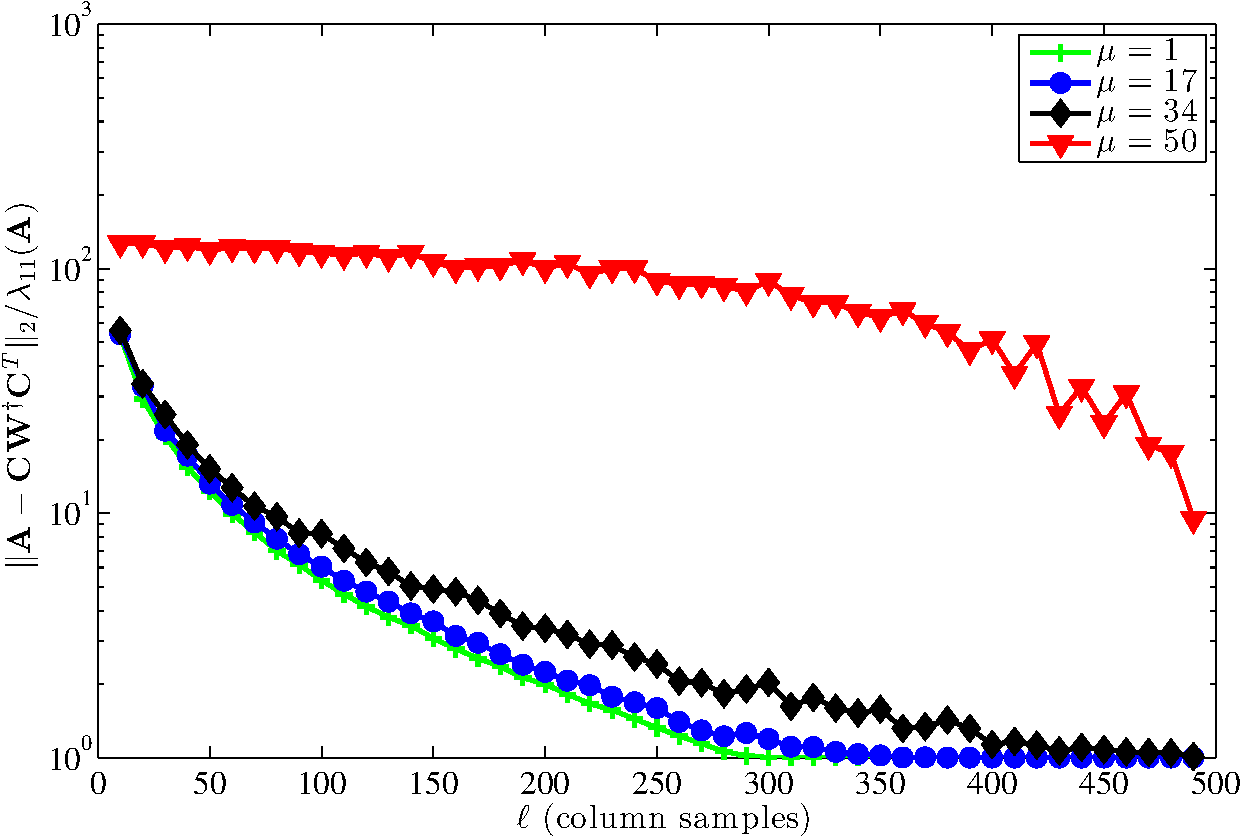
\includegraphics[width=4in,keepaspectratio=true]{nystromcoherencedependence}} 
 \end{figure}
 \vspace{-2em}
$\matA \in \R^{500 \times 500}$ is full-rank, but numerically rank 20. The target rank $k = 10.$
Each point is the average of 60 trials.

%and plot the relative spectral 
%error of the Nystr\"om extensions ($\|\matA - \matC \matW^\pinv \matC\transp\|_2 / \|\matA - \matA_k\|_2$) 
%as $\ell$ varies.

\end{frame}

 \begin{frame}
 The best previous error bound on the error of Nystr\"om extensions in terms of the coherence is 
 
 \begin{block}{\refer{Talwalkar and Rostamizadeh 2010}}
  Let $\mat{A}$ be exactly rank-$k$. If $\ell = \Omega(\mu k \log(k/\delta)),$ then 
  \[ \|\mat{A} - \mat{C} \mat{W}^\pinv \mat{C}\transp\| = 0 \]
  with probability at least $1-\delta.$
 \end{block}

 What about $\matA$ that are not exactly low-rank?
 \end{frame}
 
 \begin{frame}{Error bounds for Nystrom extensions}
  The approximation errors can be bounded when $\ell$ is proportional to the coherence.
  
  \begin{block}{Spectral-norm error bound \refer{G. 2011}}
   If $\ell \geq 8 \mu k \log(k/\delta),$ then
   \[ \|\mat{A} - \mat{C} \mat{W}^\pinv \mat{C}\transp\|_2 \leq \|\matA - \matA_k\|_2 \left(1 + \frac{2 n}{\ell} \right)\]
   with probability at least $1 - \delta.$ 
   %and
  % \[ \|\mat{A} - \mat{C} \mat{W}^\pinv \mat{C}\transp\|_2 \leq \|\matA - \matA_k\|_2 +
  %  \left( \frac{2}{\delta^2} \tr((\matA - \matA_k)^{2p-1}) \right)^{1/(2p-1)}\]
  % with probability at least $1 - 2\delta.$
  \end{block}

  This bound is \textbf{tight}: there are matrices for which the relative
  spectral-norm error is on the order of $n/\ell.$
 \end{frame} 

%  \begin{frame}
%   \begin{block}{Frobenius- and trace-norm error bounds \refer{G. and Mahoney 2013}}
%    If $\ell \geq 8 \mu k \log(k/\delta),$ then
%    \[
%     \|\matA - \matC \matW^\pinv \matC\transp\|_\rf \leq  \|\matA - \matA_k\|_\rf + \frac{4}{\delta^2}  \tr(\matA - \matA_k)
%    \]
%    and
%    \[
%     \tr(\matA - \matC \matW^\pinv \matC\transp) \leq \left(1 + \frac{2}{\delta^2}\right) \tr(\matA - \matA_k)
%    \]
%    hold simultaneously with probability at least $1 - 4\delta.$
%   \end{block}
% 
%  \end{frame}


 \begin{frame}{Conclusion}
  Considered two classes of low-rank approximation:
  \begin{enumerate}
   \item A fast projection-based scheme for arbitrary matrices.
    \begin{itemize}
     \item Established a relative-error Frobenius-norm error bound and an improved
  additive-error spectral-norm bound.
      \item Provided empirical evidence that $\Omega(k \log n)$ samples suffice to 
      obtain small spectral- and Frobenius-norm errors in practice.
    \end{itemize}

   \item A new class of SPSD sketches.
   \begin{itemize}
    \item Introduced leverage score sketches and provided empirical evidence they
     outperform alternative sketches.
     \item Provided theoretical error guarantees for several types of SPSD sketches.
     \item Established an optimal relative-error spectral-norm bound for Nystr\"om extensions.
     \item Provided empirical evidence that SPSD sketches perform well on a wide range of matrices
     that arise in machine learning.
    \end{itemize}
  \end{enumerate}

  
 \end{frame}

% \begin{frame}
%  Given the above observation, the bounds for the simple Nystr\"om extension imply the following bound on the randomized projection methodology when $\mat{S}$ selects columns
%  
%  \begin{block}{G., 2011}
%   If $\ell = \Omega(\mu k \ln(k/\delta)),$ then
%    \[ \snorm{\mat{A} - \mat{P}_{\mat{A}\mat{S}} \mat{A}} \leq \sqrt{1 + \frac{2 n}{\ell}} \cdot \snorm{\mat{A} - \mat{A}_k}  \]
%    with probability at least $1 - \delta.$
%  \end{block}
% 
%  This bound is again tight. (Note the resemblance to the Halko et al. result on the error when $\mat{S}$ is sampled from the subsampled randomized unitary transformation model)
% \end{frame}

% \begin{frame}
% Three factors determine probability of success:
% 
% \begin{itemize}
%  \item Spectral decay
%  \centerline{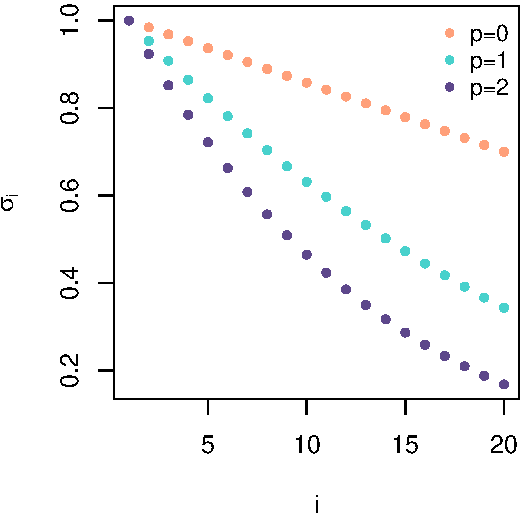
\includegraphics[scale=.7]{powermethodillust}}
% \end{itemize}
% 
% \end{frame}
% 
% \begin{frame}
% \begin{itemize}
%  \item Type of randomness
%  \vskip1em
%  \centerline{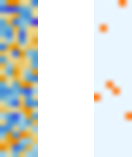
\includegraphics{samplingschemesillust}}
%  \vskip1em
%  \item Amount of oversampling (as $\ell \rightarrow n, \mat{P}_{\mat{A} \mat{S}} \rightarrow \mat{A}$)
% \end{itemize}
% 
% \end{frame}

% \subsection{Distance between subspaces}
% \begin{frame}
%  How do we measure distances between subspaces? 
% In the simplest case, two unit vectors $\mat{x}, \mat{y},$ the sine of the angle between $\mat{x}$ and $\mat{y}$ is a metric.
% \begin{columns}
% \begin{column}{.4\hsize}
%    \begin{align*}
%   \sin(\mat{x}, \mat{y})^2 & = 1 - (\mat{x}^\transp \mat{y})^2 \\
%    & = 1 - \mat{x}^\transp \mat{y} \mat{y}^\transp \mat{x} \\
%    & = \snorm{\mat{x}^\transp ( \mat{I} - \mat{y}\mat{y}^\transp) \mat{x}} \\
%    & = \snorm{\mat{x}^\transp \mat{P}_{\mat{y}^\perp} \mat{x}} \\
%    & = \snorms{\mat{P}_{\mat{y}^\perp} \mat{x}} = \snorms{\mat{P}_{\mat{y}^\perp} \mat{P}_{\mat{x}} }
%  \end{align*}
% \end{column}
% \begin{column}{.4\hsize}
%  \centerline{\includegraphics[scale=.75]{2dsineillust}}
% \end{column}
% 
% \end{columns}
% 
% \end{frame}
% 
% \begin{frame}
%  We define $\sin(\mathcal{X}, \mathcal{Y}) = \|\mat{P}_{\mathcal{X}^\perp} \mat{P}_{\mathcal{Y}}\|.$ This is not a metric in general, but always measures how much $\mathcal{X}$ contains $\mathcal{Y}.$
%   \vskip1em
%  \centerline{\includegraphics{ndsinecase1illust}\hfill\includegraphics{ndsinecase2illust}\hfill\includegraphics{ndsinecase3illust}}
%  \vskip1em
%  If $\dim(\mathcal{X}) = \dim(\mathcal{Y}),$ then $\sin$ is a metric, and 
%  \[
%   \sin(\mathcal{X}, \mathcal{Y}) = \snorm{\mat{P}_{\mathcal{X}} - \mat{P}_{\mathcal{Y}}}.
%  \]
% 
% \end{frame}
% 
% %%%%%%%%%%%%%%%%%%%%%%%%%%%%%%%%%%%%%%%%%%%%%%%%%%%%%%
% %%%%%%%%%%%%%%%%%%%%%%%%%%%%%%%%%%%%%%%%%%%%%%%%%%%%%%
% \section{\scshape Results}
% 
% %%%%%%%%%%%%%%%%%%%%%%%%%%%%%%%%%%%%%%%%%%%%%%%%%%%%%%
% %%%%%%%%%%%%%%%%%%%%%%%%%%%%%%%%%%%%%%%%%%%%%%%%%%%%%%
% \subsection{Prior results}
% \begin{frame}
% 
% Recent results (e.g. Halko et al. 2011 and Boutsidis et al. 2011)
%  \begin{block}{Norm Accuracy Results}
%  Write $\mat{A} = \mat{U}_1 \bm{\Sigma}_1 \mat{V}_1^\transp + \mat{U}_2 \bm{\Sigma}_2 \mat{V}_2^\transp.$ If $\mat{V}_1^\transp \mat{S}$ has row-rank $k,$ then
%   \[
%   \snorm{\mat{A} - \mat{P}_{\mat{A}\mat{S}} \mat{A} } \leq \sigma_{k+1}(\mat{A}) \cdot(1 + \snorm{\mat{V}_2^\transp \mat{S} (\mat{V}_1^\transp \mat{S})^\pinv})
%  \]
% \end{block}
% 
%  Obtain low error with high probability, using appropriate choices of $\mat{S},$ e.g.
%  \begin{itemize}
%   \item Gaussians with $\ell \approx k \log k$
%   \item Randomized Unitary transformations $ \ell \approx k \log n$ (sometimes)
%  \end{itemize}
%  
% \end{frame}
% 
% %%%%%%%%%%%%%%%%%%%%%%%%%%%%%%%%%%%%%%%%%%%%%%%%%%%%%%
% %%%%%%%%%%%%%%%%%%%%%%%%%%%%%%%%%%%%%%%%%%%%%%%%%%%%%%
% 
% \begin{frame}{Prior results on subspace accuracy}
%  Apply to two-sided approximations of \emph{symmetric} matrices:
%  \[ 
%     \mat{A} \approx \mat{P}_{\mat{A}\mat{S}} \mat{A} \mat{P}_{\mat{A}\mat{S}}.
%  \]
% 
% Setting:
%  \begin{align*}
%   \mat{A} & = [\mat{U}_1 \ \ \mat{U}_2] \left[\begin{matrix} \bm{\Sigma}_1 & \\ & \bm{\Sigma}_2 \end{matrix} \right] [\mat{U}_1 \ \ \mat{U}_2]^\transp \\
%   \mat{B} & = [\tilde{\mat{U}}_1 \ \ \tilde{\mat{U}}_2] \left[\begin{matrix} \tilde{\bm{\Sigma}}_1 & \\ & \tilde{\bm{\Sigma}}_2 \end{matrix} \right] [\tilde{\mat{U}}_1 \ \ \tilde{\mat{U}}_2]^\transp 
%  \end{align*}
%  
% \end{frame}
% 
% \begin{frame}
% \begin{block}{Davis--Kahan sin$\Theta$ Theorem}
%  If $\lambda(\bm{\Sigma}_1) \subseteq [a, b]$ and $\lambda(\tilde{\bm{\Sigma}}_2) \subset \overline{[a - \delta, b+ \delta]}$ then 
%  \[
%   \sin(\tilde{\mat{U}}_1, \mat{U}_1) \leq \frac{1}{\delta} \snorm{\mat{A} - \mat{B}}.
%  \]
%  \end{block}
% \vfill
%  \centerline{\includegraphics{daviskahannumberlineillust}}
% \vfill
% \end{frame}
% 
% \begin{frame}
% For randomized projections, 
% \[
% [a,b] = [\lambda_1(\mat{A}), \lambda_k(\mat{A})].
% \]
% Need
% \[
% \lambda(\tilde{\bm{\Sigma}}_2) \subset \overline{[ \lambda_1(\mat{A}) - \delta, \lambda_k(\mat{A}) + \delta]}, 
% \]
% or equivalently, $\lambda_{k+1}(\mat{B}) \geq \lambda_k(\mat{A}) + \delta.$
% 
% \end{frame}
% 
% \begin{frame}
% Applying Davis--Kahan,
% 
% \begin{align*}
%  \sin(\tilde{\mat{U}}_1, \mat{U}_1) & \leq \frac{\snorm{\mat{A} - \mat{P}_{\mat{A}\mat{S}} \mat{A} \mat{P}_{\mat{A}\mat{S}}}}{\lambda_k(\mat{A}) - \lambda_{k+1}(\mat{P}_{\mat{A}\mat{S}} \mat{A} \mat{P}_{\mat{A}\mat{S}})} \\
%   & \leq \frac{\snorm{\mat{A} - \mat{P}_{\mat{A}\mat{S}} \mat{A} \mat{P}_{\mat{A}\mat{S}}}}{(\lambda_k(\mat{A}) - \lambda_{k+1}(\mat{A})) - \snorm{\mat{A} - \mat{P}_{\mat{A}\mat{S}} \mat{A} \mat{P}_{\mat{A}\mat{S}}}}.
% \end{align*}
% 
% But we know
% \[
%   \snorm{\mat{A} - \mat{P}_{\mat{A}\mat{S}} \mat{A} \mat{P}_{\mat{A}\mat{S}}} = \mathrm{O}(\lambda_{k+1}(\mat{A})).
% \]
% 
% So Davis--Kahan applies only if
% \[
%  \lambda_k(\mat{A}) - \lambda_{k+1}(\mat{A}) = \mathrm{O}(\lambda_{k+1}(\mat{A}))
% \]
% \end{frame}
% 
% \subsection{Accuracy of randomized projections }
% \begin{frame}{Main Result}
% 
% \begin{block}{Subspace approximation with random projections}
% Let $\tilde{\mat{A}} := (\mat{A}\mat{A}^\star)^p \mat{A}.$ Then, if $\mat{V}_1^\transp \mat{S}$ has full row-rank, 
% \[
% \sin(\mat{A}_k, \left[\mat{P}_{\tilde{\mat{A}} \mat{S}} \tilde{\mat{A}} \right]_k) \leq \left(\frac{\sigma_{k+1}}{\sigma_k}\right)^{2p+1} (1 + \sqrt{2} + \sqrt{2} \snorm{\mat{V}_2^\transp \mat{S} (\mat{V}_1^\transp \mat{S})^\pinv})
% \]
% \end{block}
% 
% Accuracy depends on
% \begin{itemize}
%  \item spectral decay (\emph{ratio}, potentially enchanced by power method)
%  \item type of randomness 
%  \item amount of oversampling
% \end{itemize}
% 
% Cost of approximation is $\mathrm{O}(mnlp)$
% \end{frame}
% 
% \begin{frame}
%  The interaction term $\snorm{\mat{V}_2^\transp \mat{S} (\mat{V}_1^\transp \mat{S})^\pinv}$ is ``inherited'' from analyses of the norm error
%  \begin{itemize}
%   \item is it necessary?
%   \item is it natural (geometric)?
%  \end{itemize}
% 
%  How tight is this bound?
% \end{frame}
% 
% %%%%%%%%%%%%%%%%%%%%%%%%%%%%%%%%%%%%%%%%%%%%%%%%%%%%%%
% %%%%%%%%%%%%%%%%%%%%%%%%%%%%%%%%%%%%%%%%%%%%%%%%%%%%%%
% \subsection{A new analysis of the subspace iteration method}
% 
% \begin{frame}{Column-based approximations}
% Consider first how much of the range of $\mat{A}_k$ is contained in that of $\mat{A}\mat{S}$
% 
% \begin{block}{Subspace containment}
% Let $\mat{S} \in \R^{n \times \ell}$ be such that $\mat{V}_1^\transp \mat{S}$ has rank $k$, then
% \[
%  \sin^2(\mat{A} \mat{S}, \mat{A}_k) = 1 - \lambda_k\left(\big(\mat{S}^\transp \mat{A}^\transp \mat{A} \mat{S}\big)^\pinv \mat{S}^\transp \mat{A}_k^\transp \mat{A}_k \mat{S} \right)
% \]
% \end{block}
% 
% Note 
% \[
%  \mat{S}^\transp \mat{A}^\transp \mat{A} \mat{S} = \mat{S}^\transp \mat{A}_k^\transp \mat{A}_k \mat{S} + \mat{E}.
% \]
% 
% \end{frame}
% 
% \begin{frame}[Subspace iteration method]
% 
% It follows that if $\mat{S}$ has $k$ columns, then 
% \begin{block}{Accuracy of subspace iteration}
% \[
%  \sin((\mat{A}\mat{A}^\star)^p \mat{A} \mat{S}, \mat{A}_k) = \frac{\gamma_p^2 }{1 + \gamma_p^2}
% \]
% where 
% \[
%  \gamma_p = \snorm{\bm{\Sigma}_2^{2p+1} \cdot \mat{V}_2^\transp \mat{S} (\mat{V}_1^\transp \mat{S})^\pinv  \cdot \bm{\Sigma}_1^{-(2p+1)}}.
% \]
% \end{block}
% 
% Gives the \emph{exact} error of the classical subspace iteration method.
% 
% \end{frame}
% 
% \begin{frame}
%  Classical error bound for subspace iteration method:
%  \[
%   \tan(\mat{A}^p \mat{S}, \mat{A}_k)\leq \left| \frac{\lambda_{k+1}}{\lambda_k} \right|^p \tan(\mat{S}, \mat{A}_k), 
%  \]
% where
% \[
%  \tan(\mat{S}, \mat{V}_1) = \frac{\sin(\mat{S}, \mat{V}_1)}{\cos(\mat{S}, \mat{V}_1)} = \frac{\snorm{\mat{P}_{\mat{S}} - \mat{P}_{\mat{V}_1}}}{\sqrt{1 - \snorms{\mat{P}_{\mat{S}} - \mat{P}_{\mat{V}_1}}}}.
% \]
% implies
% \[
%  \sin(\mat{A}^p \mat{S}, \mat{A}_k) \leq \left| \frac{\lambda_{k+1}}{\lambda_k} \right|^p \sin(\mat{S}, \mat{A}_k).	
% \]
% 
% \end{frame}
% 
% \subsection{The geometry of randomized projections}
% \begin{frame}
%  \begin{block}{Geometry of randomized projections}
%  WLOG, assume $\mat{S}$ has orthonormal columns. Then $\mat{V}_1^\transp \mat{S}$ has full row rank iff 
%  \[
%   \sin(\mat{V}_1, \mat{S}) < 1
%  \]
%  and if this holds, then
%  \[
%   \snorm{\mat{V}_2^\transp \mat{S} (\mat{V}_1^\transp \mat{S})^\pinv} = \tan(\mat{V}_1, \mat{S}).
%  \]
%  \end{block}
%  
%  \begin{itemize}
%   \item The quantity of interest in randomized projection-based low-rank approximations, $\snorm{\bm{\Sigma}_2^{2p+1} \cdot \mat{V}_2^\transp \mat{S} (\mat{V}_1^\transp \mat{S})^\pinv  \cdot \bm{\Sigma}_1^{-(2p+1)}}$ is a ``weighted'' tangent.
%   \item Allows exact bounds on the quantity $\snorm{\mat{V}_2^\transp \mat{S} (\mat{V}_1^\transp \mat{S})^\pinv}$ for sampling with Gaussian vectors.
%  \end{itemize}
%  
%  \end{frame}
%  
%  \begin{frame}
% Allows bounding the angle between fixed subspaces and highly \emph{nonuniformly} distributed random subspaces, e.g.
%  \[
%   \sin(\mat{V}_1, \mat{S}) \leq \frac{n}{n + \ell \varepsilon} \text{ w. p. } > 1-\delta \text{ when } \ell \geq  \mu(\mat{V}_1)  \delta^{-1} \varepsilon^{-2} k \log k.
%  \]
%  when $\mat{S}$ is a random axis-aligned $\ell$-dimensional subspace.
% \end{frame}
% 
% \begin{frame}
%  When $\ell = k,$ 
%  \[
%    \mat{P}_{\left[\mat{P}_{(\mat{A}\mat{A}^\star)^p \mat{A}\mat{S}} (\mat{A}\mat{A}^\star)^p \mat{A} \right]_k} =
%    \mat{P}_{(\mat{A}\mat{A}^\star)^p \mat{A}\mat{S}},
%  \]
% so the randomized projection method \emph{is} subspace iteration.
% Comparison of bounds:
% \begin{itemize}
%  \item Subspace iteration: 
%  \[
%   \sin(\mat{A}_k, (\mat{A}\mat{A}^\star)^p \mat{A}\mat{S}) \leq 
%   \left(\frac{\sigma_{k+1}}{\sigma_k}\right)^{2p+1} \cdot \frac{\tan(\mat{S}, \mat{V}_1)}{\left(\frac{\sigma_k}{\sigma_{k+1}}\right)^{2p+1} + 
%   \tan(\mat{S}, \mat{V}_1)}
%  \]
% 
%  \item Randomized projection method:
%  \[
%   \sin(\mat{A}_k, (\mat{A}\mat{A}^\star)^p \mat{A}\mat{S}) \leq \left(\frac{\sigma_{k+1}}{\sigma_k}\right)^{2p+1} \cdot (1 + \sqrt{2} + \sqrt{2} \cdot \tan(\mat{S}, \mat{V}_1) )
%  \]
% 
% \end{itemize}
% 
% \end{frame}
% 
% \begin{frame}{What we would really like to do}
% Take $\ell > k$ samples and consider how well $[\mat{A}\mat{S}]_k$ approximates the range of $\mat{A}_k$
% 
% \begin{block}{Subspace iteration with oversampling}
% Let $\mat{S} \in \R^{n \times \ell}$ be such that $\mat{V}_1^\transp \mat{S}$ has rank $k$, then
% \[
%  \sin^2([\mat{A} \mat{S}]_k, \mat{A}_k) = 1 - \lambda_k\left(\big(\big[\mat{S}^\transp \mat{A}^\transp \mat{A} \mat{S}\big]_k\big)^\pinv \mat{S}^\transp \mat{A}_k^\transp \mat{A}_k \mat{S} \right)
% \]
% \end{block}
% 
% \end{frame}
% 
% %%%%%%%%%%%%%%%%%%%%%%%%%%%%%%%%%%%%%%%%%%%%%%%%%%%%%%
% %%%%%%%%%%%%%%%%%%%%%%%%%%%%%%%%%%%%%%%%%%%%%%%%%%%%%%
% \section{\scshape Applications}
% 
% \subsection{Approximate leverage scores}
% \begin{frame}{Leverage score approximation}
% The statistical leverage scores of the columns of $\mat{A}$ (w.r.t to rank $k$), are the column norms
% \[
%  \{ \ell_j := \snorms{(\mat{V}_1)_j}, j=1,\ldots,m \}.
% \]
% \vfill
% \centerline{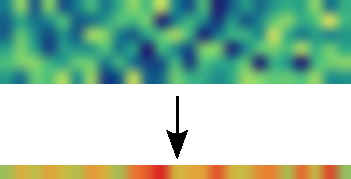
\includegraphics{levscoresillust}}
% \vfill
% 
% \end{frame}
% 
% \begin{frame}
% Exposes the natural nonuniformity structure in $\mat{A}:$
% \[
%  \mat{A}_j = \sum_{i=1}^{\rank(\mat{A})} \sigma_i (\mat{u}_i \mat{v}_i^t)_j = \sum_{i=1}^k \sigma_i (\mat{V}_1)_{ji} \mat{u}_i + \cdots
% \]
% so
% \[
%  \ell_j = \snorms{(\mat{V}_1)_j} = \sum_{i=1}^k (\mat{V}_1)_{ji}^2 
% \]
% reflects how much $\mat{U}_1$ is determined by $\mat{A}_j.$
% 
% \end{frame}
% 
% \begin{frame}
%  Useful in
% \begin{itemize}
%  \item statistics (outlier identification)
%  \item matrix completion
%  \item column-sampling based low-rank approximations
% \end{itemize}
% 
% \end{frame}
% 
% \begin{frame}
% Drineas et al. 2011 propose following algorithm for approximating leverage scores:
% \begin{itemize}
%   \item Let $S$ be in $\R^{n \times (2k)}$ with i.i.d. $\mathcal{N}(0,1)$ entries
%   \item Compute $\mat{Y} = (\mat{A} \mat{A}^\star)^p \mat{A} \mat{S}$ 
%   \vskip0.5em
%   \centerline{\includegraphics{drineasleveragescorealgillust}}
%   \vskip0.5em
%   \item Approximate the leverage scores of $\mat{A}$ with those of $\mat{Y}.$
% \end{itemize}
% Do not prove a relationship between leverage scores of $\mat{A}$ and $\mat{Y}.$
% 
% \end{frame}
% 
% \begin{frame}{Analysis of Drineas et al.'s algorithm}
%  
%  \begin{itemize}
%   \item Let $\tilde{\mat{V}}_1$ contain the top $k$ right singular vectors of $Y.$
%   \item Note that $\snorms{(\mat{V}_1)_j} = (\mat{V}_1 \mat{V}_1^\transp)_{jj} = (\mat{P}_{\mat{V}_1})_{jj}.$
%  % put illustrations here showing that the leverage scores determined by the diagonal entries of the projections
%  \item Thus the approximation errors all satisfy
%   \begin{align*}
%    | \ell_j - \tilde{\ell}_j | & = | (\mat{P}_{\mat{V}_1})_{jj} - (\mat{P}_{\tilde{\mat{V}}_1})_{jj} | 
%    \leq \snorm{\mat{P}_{\mat{V}_1} - \mat{P}_{\tilde{\mat{V}}_1}} \\
%     & \leq \left(\frac{\sigma_{k+1}}{\sigma_k}\right)^{2p+1} \cdot( 1 + \sqrt{2} + \sqrt{2} \tan(\mat{S}, \mat{V}_1))
%   \end{align*}
%  \end{itemize}
%  
% \end{frame}
% 
% \begin{frame}[fragile]{Spectral Clustering}
% Given data points $\{\mat{x}_j\}_{i=1,\ldots, n},$ want to form $k$ clusters using information in similarity graph.
% 
%  Prototypical algorithm:
%  
%   \begin{algorithm}[H]
%   \renewcommand{\alglinenumber}[1]{\tiny #1.} 
%   \scriptsize
%   \begin{algorithmic}[1]
%   \State Form affinity matrix 
%   \[
%     \mat{W}_{ij} = \begin{cases} \exp(-\snorm{\mat{x}_i - \mat{x}_j}/\sigma)& i \neq j \\
%                     0 & i = j
%                    \end{cases}
%   \]
%   and diagonal matrix
%   \[
%     \mat{D}_{ii} = \sum_{j=1}^n \mat{W}_{ij}
%   \]
%   \State Form a Laplacian
%   \[
%     \mat{L} = \mat{D} - \mat{W}.
%   \]
%   \State Take $\mat{L} = \mat{U} \bm{\Sigma} \mat{U}^\transp.$ 
%   \State Perform $k$-means clustering on the rows of $\mat{U}_1.$ 
%   \State Assign data points $\mat{x}_i$ and $\mat{x}_j$ to the same cluster iff rows $i$ and $j$ were clustered together. 
%   \end{algorithmic}
%   \end{algorithm}
% \end{frame}
% 
% \begin{frame}{Approximate spectral clustering}
% Rows of $\mat{U}_1$ and $\mat{U}_1 \mat{O}$ cluster in the same way
% % illustration that rotations don't change clusterings
% \centerline{\includegraphics{clusterstability1illust}}
%  To use randomized projections to speed up spectral clustering,
%  \[
%   \inf_{\mat{O} \mat{O}^\transp = \mat{I}} \snorm{\mat{U}_1 - \tilde{\mat{U}}_1 \mat{O}} \leq \varepsilon
%  \]
%  suffices to get same clustering.
% 
% \end{frame}
% 
% \begin{frame}
%  Best analysis of randomized projections for spectral clustering (follows from Hunter and Strohmer, 2010):
%  
%  There is an $\mat{O}$ so that 
%  \[
%   \snorm{\mat{U}_1 - \tilde{\mat{U}}_1 \mat{O}} \leq (2 + 2 \sqrt{2})\frac{\fnorm{\mat{L} - \mat{L}_k}}{\lambda_k - \lambda_{k+1}}  (1 + \tan(\mat{S}, \mat{L}_k))
%  \]
% 
%  Requires approximating $\mat{L}$ with a positive matrix.
% \end{frame}
% 
% \begin{frame}
%  \begin{block}{Sharper analysis}
%  
%  There is an $\mat{O}$ so that
%  \begin{align*}
%   \snorm{\mat{U}_1 - \tilde{\mat{U}}_1 \mat{O}} & \leq \sqrt{2} \sin(\mat{U}_1, \tilde{\mat{U}}_1) \\
%   & \leq \left(\frac{\sigma_{k+1}}{\sigma_k}\right) \cdot (\sqrt{2} + 2 + 2 \cdot \tan(\mat{S}, \mat{L}_k))
%  \end{align*}
%  
%  \end{block}
%  
%  Does not require approximating $\mat{L}$ with a positive matrix.
% \end{frame}
% 
% \subsection{Regularized canonical correlation scores}
% \begin{frame}{Canonical Correlation Analysis}
%  Canonical correlation scores are the angles between subspaces $\mathcal{X}, \mathcal{Y}:$
% \vskip1em
%  \centerline{\includegraphics{ndsinecase1illust}}
%  \vskip1em
%  Used in machine learning: object recognition, image segmentation, pattern recognition, $\ldots$
% \end{frame}
% 
% \begin{frame}
% Scores given by
% \[
%  \cos \theta_i = \max_{\mat{x} \in \mathcal{X}} \max_{\mat{y} \in \mathcal{Y}} \mat{x}^\transp \mat{y} = \mat{x}_i^\transp \mat{y}_i
% \]
% for  $i=1,\ldots, \min(\dim(\mathcal{X}), \dim(\mathcal{Y})).$
%  
% Computable as 
% \[
%  \cos \theta_i = \sigma_i(\mat{Q}_{\mathcal{X}}^\transp \mat{Q}_{\mathcal{Y}}).
% \]
% 
% \end{frame}
% 
% \begin{frame}{Regularized Canonical Correlation Analysis}
%  In applications, $\mathcal{X} = \mathcal{R}(\mat{A})$ and $\mathcal{Y} = \mathcal{R}(\mat{B}).$ Scores unstable with respect to noise in $\mat{A},\mat{B}.$
%  % illustration
%  
%  Suggests regularization: use scores of $\mat{A}_k$ and $\mat{B}_r$
% \end{frame}
% 
% \begin{frame}{Approximate Regularized Canonical Correlation Analysis}
% Can use random projections to efficiently approximate regularized scores of large matrices.
% 
% \begin{block}{Accuracy of approximate regularized CCA scores}
% If $\rank(\tilde{\mat{A}}) = \rank(\mat{A}_k)$ and $\rank(\tilde{\mat{B}}) = \rank(\mat{B}_r),$ then 
% \[
% |\sigma_i(\mat{A}_k, \mat{B}_r) - \sigma_i(\tilde{\mat{A}}, \tilde{\mat{B}})| \leq \sin(\tilde{\mat{A}}, \mat{A}_k) + \sin(\tilde{\mat{B}}, \mat{B}_r)
% \]
% for $i = 1,\ldots.$
% \end{block}
% 
% Take $\tilde{\mat{A}} = \left[\mat{P}_{(\mat{A}\mat{A}^\star)^p \mat{A}\mat{S}_1} (\mat{A}\mat{A}^\star)^p \mat{A}\right]_k$ and 
% $\tilde{\mat{B}} = \left[\mat{P}_{(\mat{B}\mat{B}^\star)^p \mat{B} \mat{S}_2} (\mat{B}\mat{B}^\star)^p \mat{B}\right]_k.$
% 
% Costs $\mathrm{O}(mnlp)$ operations. 
% \end{frame}
% 
% \section{\scshape Summary}
% \begin{frame}{Summary}
%  \begin{itemize}
%   \item For spectral methods, there seems to be no advantage in using $\left[\mat{P}_{\mat{A}\mat{S}} \mat{A} \right]_k$ instead of $\left[\mat{A}\mat{S}\right]_k$ to approximate the top left invariant subspace of $\mat{A}$
%   \item A new bound which may lead to understanding of how oversampling helps with subspace iteration
%   \item A geometric interpretation of the quantity that arises in error bounds for random projection-based low-rank approximation
%   \item Analysis of several fast spectral algorithms that use subspace iteration
%  \end{itemize}
% 
% \end{frame}
% 
% \section{\scshape For future investigation}
% \begin{frame}{Research Directions}
% \begin{itemize}
% 	\item Randomized estimator for $\sin(\mat{A}, \mat{B})$?
% 	\item Analysis of power method with oversampling --- seems more appropriate/efficient since don't want $\mat{A},$ just its dominant invariant subspace
% 	\item Sharper analyses of $\tan(\mat{S}, \mat{V}_1)$ for interesting/practical choices of $\mat{S}$
% %	\item Accuracy of $\left[\mat{P}_{\mat{A} \mat{S}} \mat{A}\right]_k$ in approximating $\mat{A}_k$
% \end{itemize}
% \end{frame}
\end{document}